\documentclass[a4paper,10pt]{scrartcl}

\usepackage[utf8]{inputenc}
\usepackage[ngerman]{babel}
\usepackage[T1]{fontenc}
\usepackage{amsmath}
\usepackage[section]{placeins}
\usepackage{graphicx}
\usepackage{esvect}
\usepackage{amssymb}



\title{Praktikum B Vorbereitung zu Versuch "og"}
\author{Leon Machtl und Raphael Lehner}
\date{28.11.2019}

\begin{document}
	\maketitle
	\tableofcontents
	\newpage
	
	\section{Einleitung zum Versuch}
		In diesem Versuch wird mit einfachen, aber dennoch wichtigen Geräten experimentiert. Dabei steht die eigene Beobachtung im Vordergrund und die quantitative Auswertungen beruhen auf den Gesetzen der geometrischen Optik. Die geometrische Optik macht Gebrauch von dem sogenannten Strahlenmodell des Lichtes. Damit wird, vereinfacht ausgedrückt, der Weg des Lichtes auf Linien in rein geometrischer Weise betrachtet. So ein Linienstrahl entspricht natürlich in keiner Weise der Realität, weswegen er sich nicht experimentell realisieren lässt. Mit Hilfe der geometrischen Optik lässt sich aber dennoch die Funktion der Abbildung durch optische Geräte wie Lupen, Linsen, Brillen, Mikroskope, Fernrohre oder Teleskope häufig ausreichend genau beschreiben. Mathematisch kann man die geometrische Optik als Grenzfall für Wellenlängen, die gegen Null gehen, auffassen. Sie ist jedoch auch in dieser Betrachtungsweise nicht exakt. Effekte, die nicht mit Hilfe der geometrischen Optik beschrieben werden können, können häufig durch die Wellenoptik, beziehungsweise quantenmechanische Betrachtungen beschrieben werden. Dazu gehören beispielsweise Interferenz, Beugung, Polarisation, Absorption und Streuung des Lichtes. \\
		Im Rahmen dieses Experiments werden mehrere optische Geräte betrachtet. Bei diesen handelt es sich um die Lupe, mit der lediglich qualitative Beobachtungen durchgeführt werden sollen, das astronomische Fernrohr, das terrestrische Fernrohr, das holländische oder auf Galileische Fernrohr, sowie das Spiegelteleskop und der Diaprojektor. Dabei liegt der Fokus darin, die verwendeten Geräte selber zu bauen und ihre Wirkungsweise zu verstehen.\\
		Weitere Ziele des Versuchs sind theoretische Überlegungen und Berechnungen experimentell zu überprüfen, die Grundgesetze der geometrischen Objekt durch ihre Anwendung besser zu verstehen, Probleme der geometrischen Optik praktisch zu lösen, Versuchsaufbauten selbst zu justieren und zu optimieren und wie oben bereits erwähnt, wichtige optische Geräte und Instrumente selbst nachzubauen.
		
		\newpage
		
	\section{Fragen zur Vorbereitung}
		\subsection{Frage 1}
			Wie lautet die Abbildungsgleichung für dünne Sammel- und Zerstreuungslinsen? Welche Näherungen
			werden bei der Herleitung gemacht? Was ist die Hauptebene einer Linse?\\
			\\
			\begin{figure}[h]
\centering
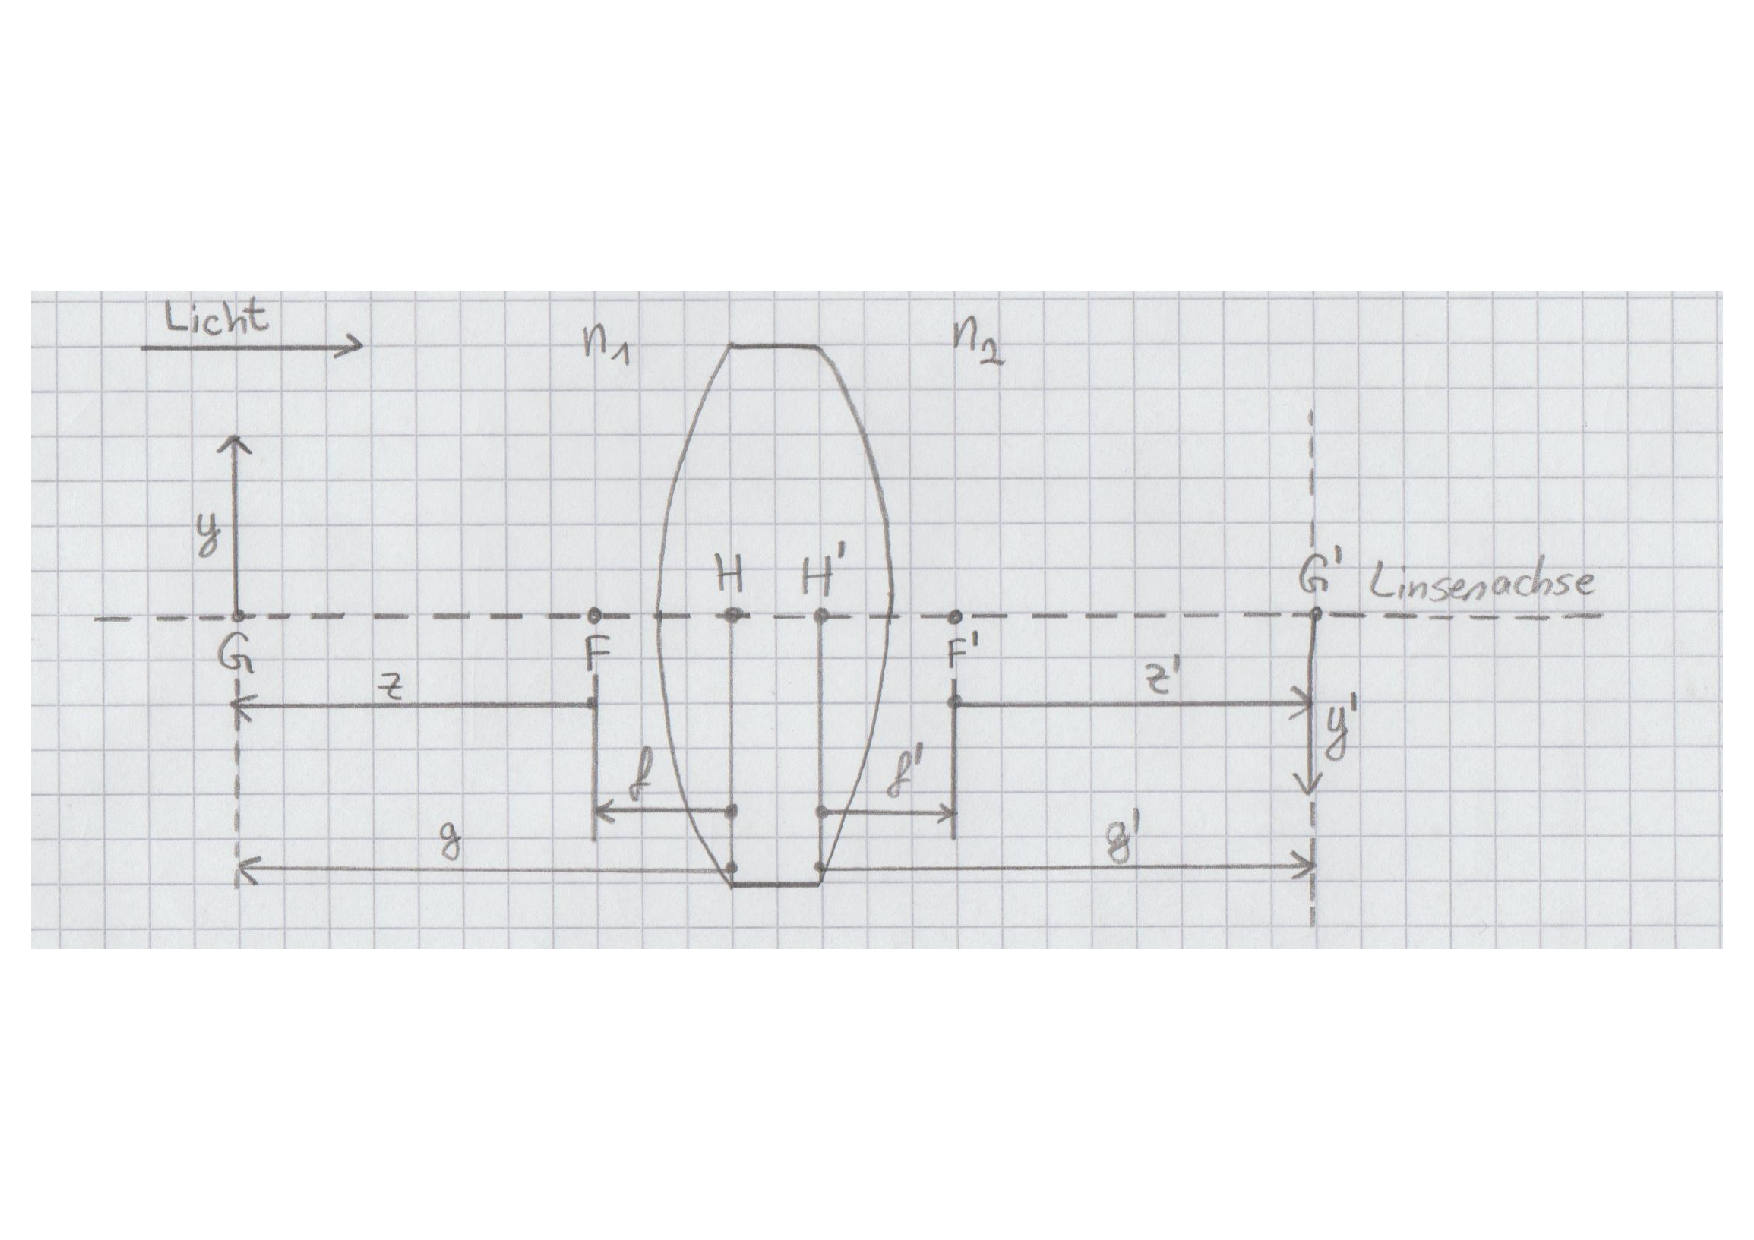
\includegraphics[width=0.9\textwidth]{./Bilder/og8}
\end{figure}
\FloatBarrier
			\\
			In der Skizze entsprechen \(f\) und \(f'\) der sogenannten Brennweite, welche wiederum den Entfernungen der Brennpunkte \(F\) und \(F'\) von den beiden Hauptpunkten \(H\) und \(H'\) der Linse entspricht. Der Brennpunkt einer Linse bezeichnet den Punkt, an dem sich parallel zur Achse der Linse einfallende Strahlen treffen. Dabei sind \(f\) und \(f'\) verschieden, wenn die beiden Medien vor und hinter der Linse verschieden sind. Eine Entfernung zu einem Gegenstand \(G\) beziehungsweise die Entfernung zu seinem Bild \(G'\) mit jeweils der Höhe \(y\), beziehungsweise \(y'\) kann entweder von den Hauptpunkten oder den Brennpunkten aus gemessen werden. Dabei bezeichnen \(g\) und \(g'\) die Entfernung von den Hauptpunkten aus gemessen (Objektweite und Bildweite) und \(z\), beziehungsweise \(z'\) die Entfernung von den Brennpunkten. Betrachtet man nun eine dünne Linse, so fallen \(H\) und \(H'\) zusammen (Schnittpunkt Hauptebene und Linsenachse). Von der Bildseite einfallende parallele Strahlen, die auf eine Sammellinse fallen, werden in \(F'\) zusammengeführt. Bei einer Zerstreuunglinse ist dies nicht der Fall, \(F'\) liegt hier vor der Linse (Vergleiche Skizze).\\
			\\
	\begin{figure}[h]
\centering
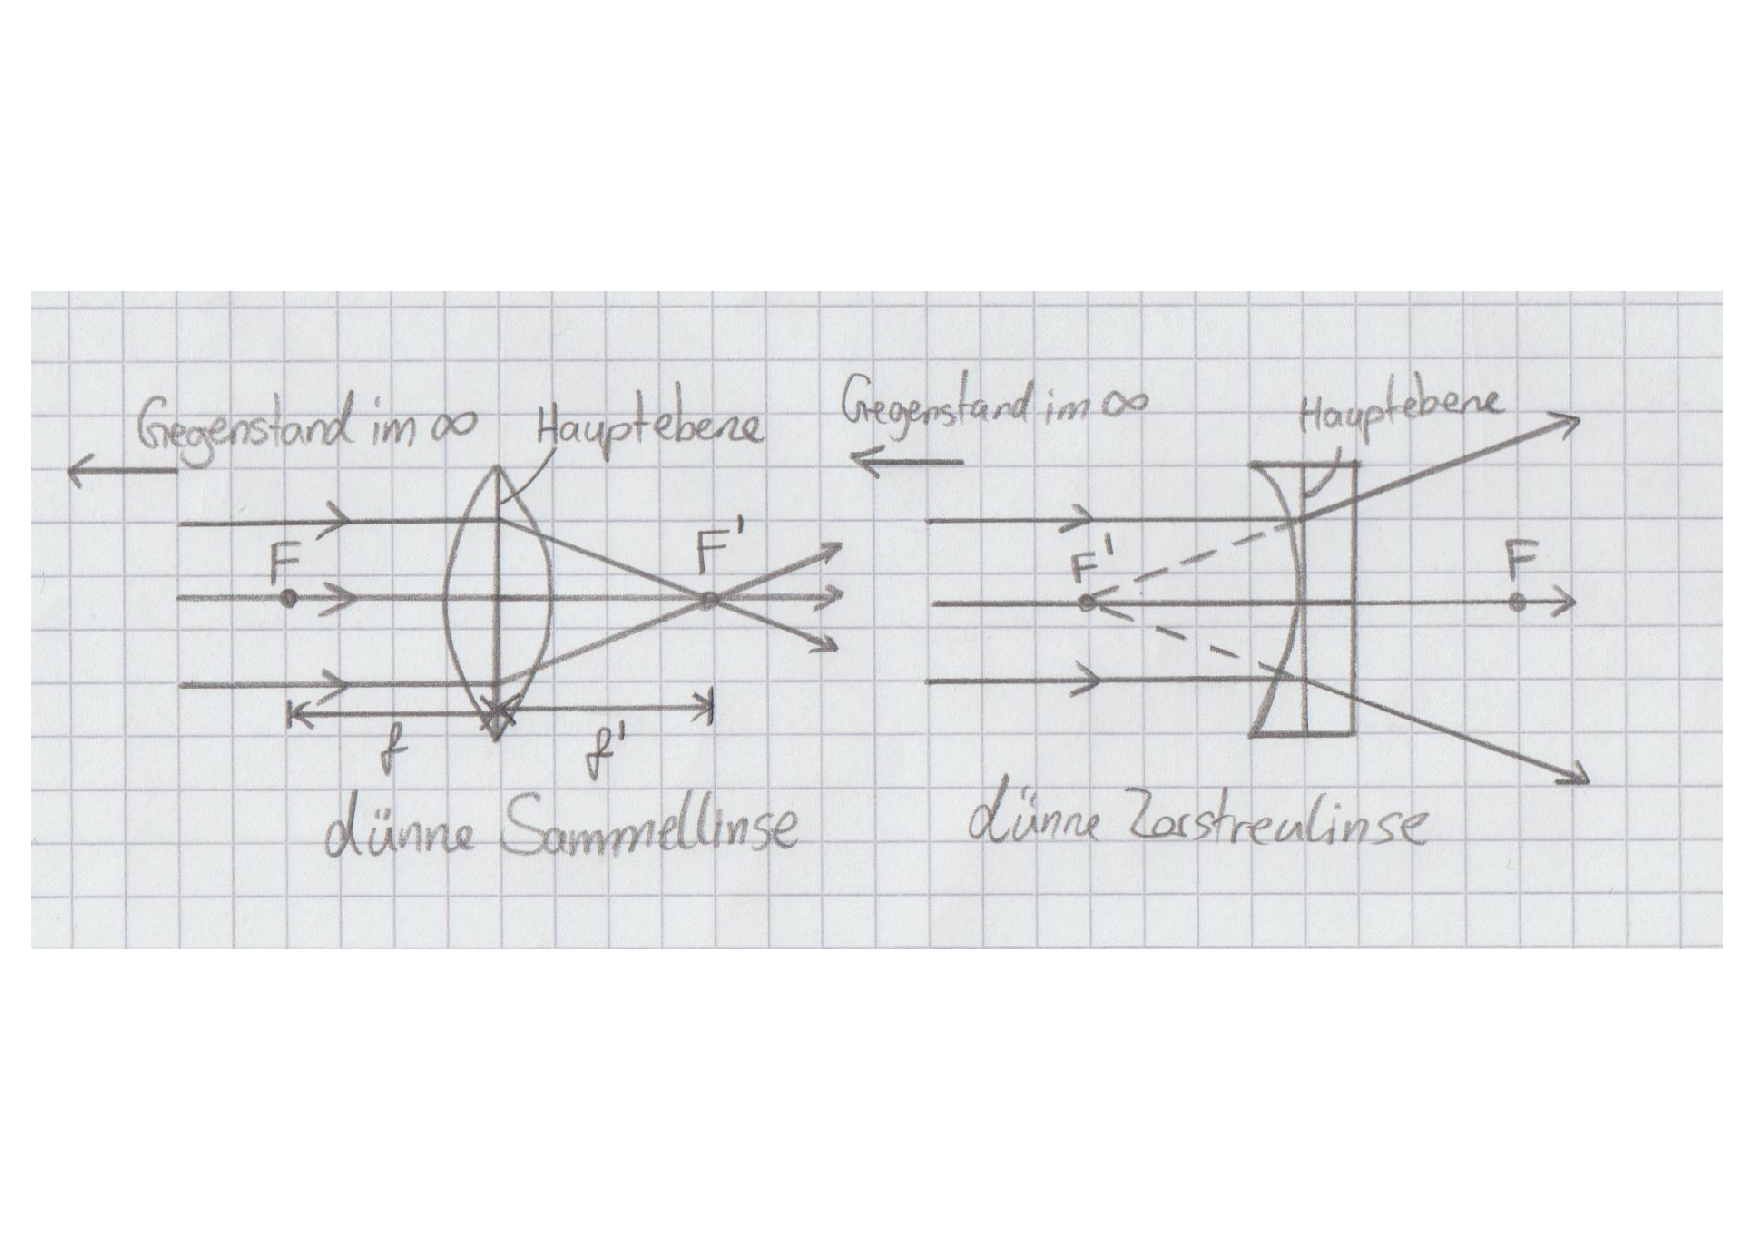
\includegraphics[width=0.9\textwidth]{./Bilder/og9}
\end{figure}
\FloatBarrier			\\
			Bei dünnen Linsen betrachtet man die Brechung näherungsweise in der Hauptebene und nicht auf der Oberfläche der Linse. Somit definiert der Brechungsindex der Linse nur eine und nicht zwei Brechungen. Diese Vereinfachung führt zu der Abbildungsgleichung für dünne Sammel- und Zerstreuunglinsen, welche durch
			\begin{align*}
			\frac{y'}{y}=\frac{g'}{g}
			\end{align*}
			ausgedrückt wird. Auch folgende Gleichung wird als Abbildungsgleichung bezeichnet:
			\begin{align*}
			\frac{1}{g}+\frac{1}{g'}=\frac{1}{f}
			\end{align*}
			
		\subsection{Frage 2}
			Wodurch werden die Bildhelligkeit und das Gesichtsfeld beeinflusst bzw. begrenzt?\\
			\\
			Die Bildhelligkeit und das Gesichtsfeld werden durch Blenden beeinflusst, beziehungsweise begrenzt. Bei einem Auge übernimmt diese Aufgabe die Pupille.
			
		\subsection{Frage 3}
			Leiten Sie die Formeln für die Vergrößerung von Lupe, den Fernrohren und dem Mikroskop
			her. Berücksichtigen Sie beim Fernrohr insbesondere die großen Gegenstandsweiten.\\
			\\
			Die Vergrößerung \(V\) eines optischen Gerätes ist definiert als
			\begin{align*}
			V=\frac{tan\epsilon}{tan\epsilon_{0}}
			\end{align*}	
			wobei \(\epsilon\) der Sehwinkel ist, unter dem das Objekt im optischen Instrument erscheint. \(\epsilon_{0}\) ist der Sehwinkel, unter dem man das Objekt ohne optische Hilfsmittel sieht. Der Winkel hängt vom Abstand des Auges zum Objekt ab und wir größer, je näher das Objekt ist. Optische Geräte, wie Lupe, Fernrohre und das Mikroskop dienen nun dazu, den Sehwinkel unter dem das Auge weit entfernte Objekte sieht, zu Vergrößern. Um die Winkelvergrößerung zu berechnen, wurde eine Bezugsweite von \(S=250mm\) definiert, bei der man Gegenstände mit bloßem Auge scharf sehen könnte.\\
			\\
			Lupe:\\
			\\
			Eine Lupe mit einer kurzen Brennweite ermöglicht die Betrachtung von kleinen Objekten mit Höhe \(y\) in der Entfernung \(s\) mit \(s<<S\) Der Abstand zwischen Auge und Objekt ist kleiner als \(2f\), wobei f wie oben der Brennweite entspricht. Die Situation ist in folgender Skizze ersichtlich:\\
			\\
				\begin{figure}[h]
\centering
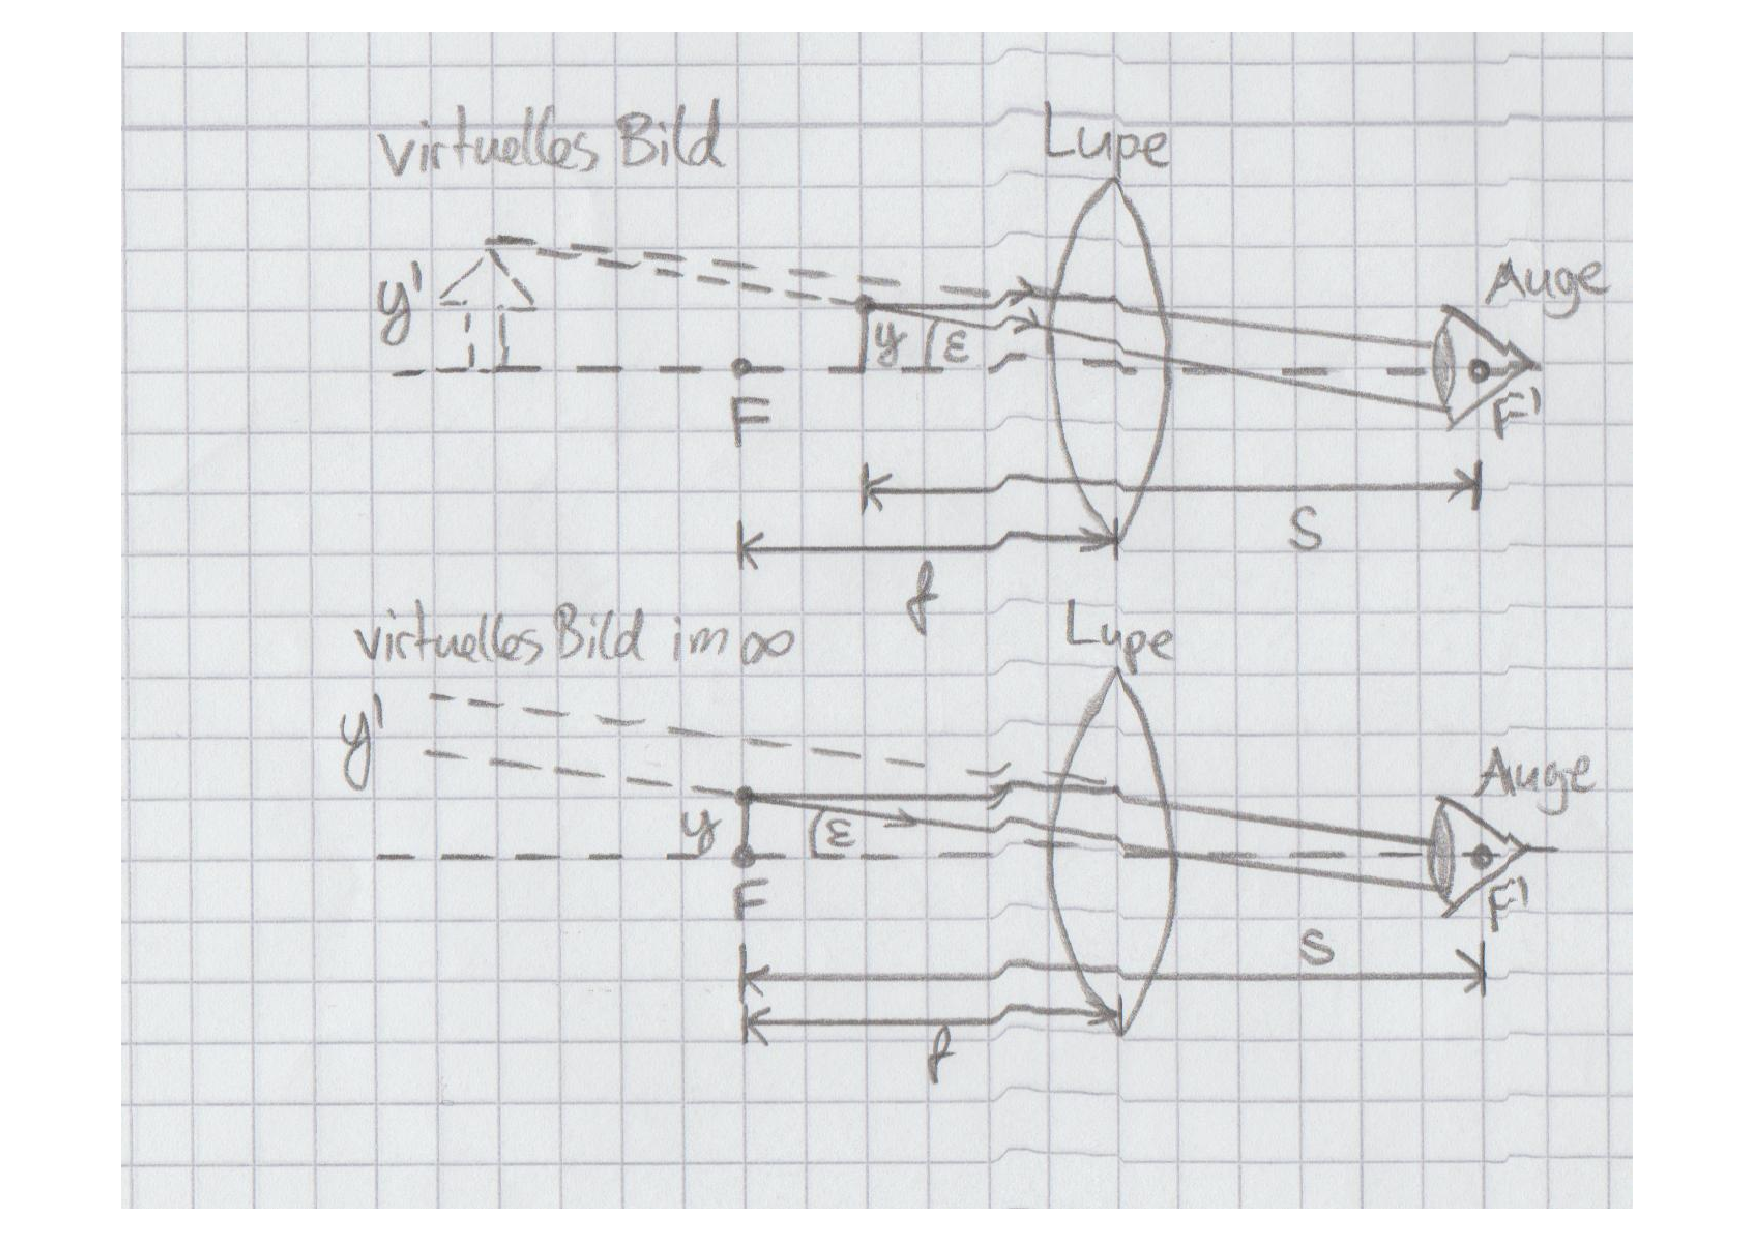
\includegraphics[width=0.9\textwidth]{./Bilder/og4}
\end{figure}
\FloatBarrier
			\\
			Man kann ein virtuelles Bild mit Höhe \(y'\) beobachten. Befindet sich das Objekt genau in der Brennebene, so liegt \(y'\) im Unendlichen. In diesem Fall beträgt die Vergrößerung der Lupe
			\begin{align*}
			V_{L}=\frac{tan\epsilon}{tan\epsilon_{0}}=\frac{\frac{y}{f}}{\frac{y}{S}}=\frac{S}{f}
			\end{align*}
			\\
			Fernrohr:\\
			\\
			Bei einem astronomischen Fernrohr\\
			\\
	\begin{figure}[h]
\centering
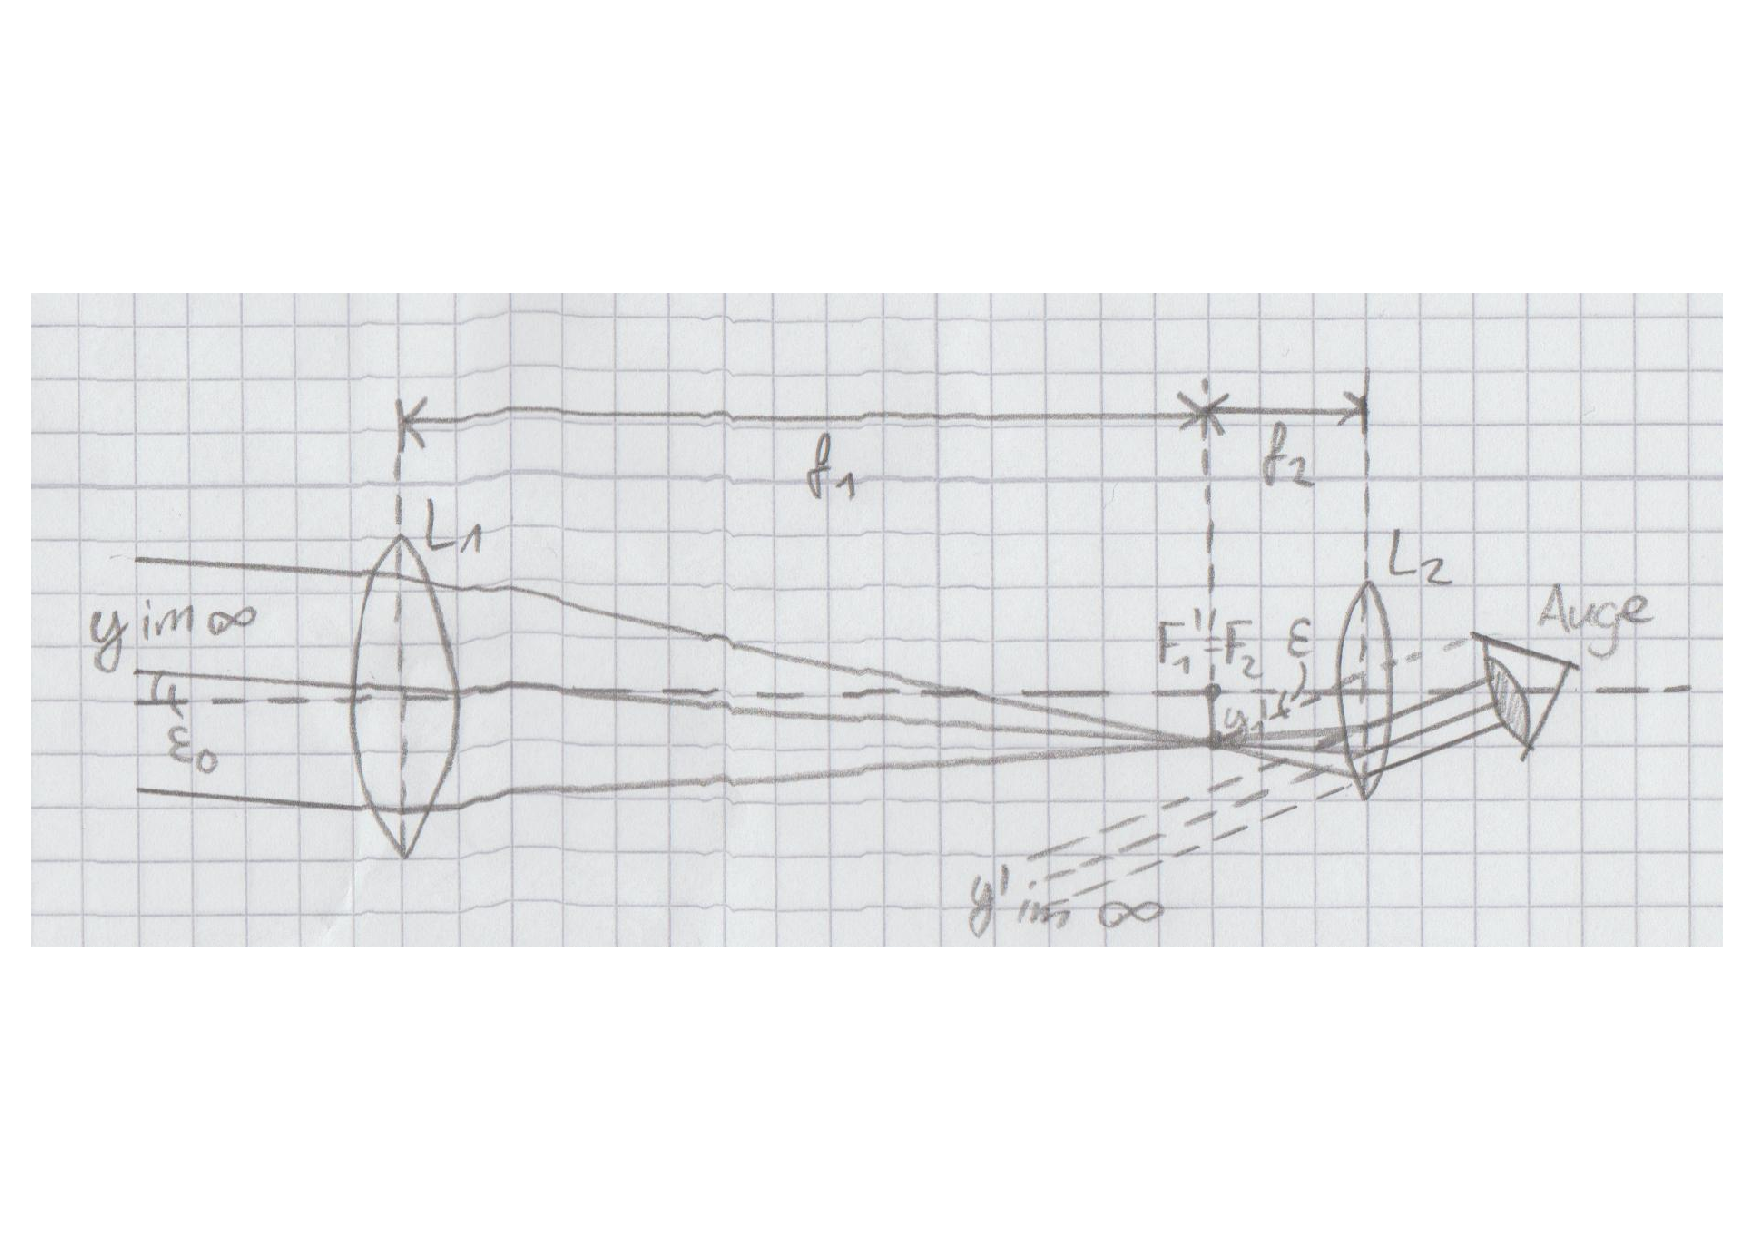
\includegraphics[width=0.9\textwidth]{./Bilder/og5}
\end{figure}
\FloatBarrier			\\
			wird durch die Linse \(L_{1}\) von einem näherungsweise unendlich weit entfernten Objekt mit Höhe \(y\) ein umgekehrtes Bild der Höhe \(y'\) in der Brennebene erzeugt. Dabei handelt es sich um ein sogenanntes Zwischenbild, welches durch eine Linse \(L_{2}\) als virtuelles Bild im Unendlichen betrachtet wird, wenn \(F'_{1}=F_{2}\). In diesem Fall folgt für die Vergrößerung des astronomischen oder auch Keplerfernrohres
			\begin{align*}
			V_{kep}=\frac{tan\epsilon}{tan\epsilon_{0}}=\frac{\frac{y'_{1}}{f_{2}}}{\frac{y'_{1}}{f_{1}}}=\frac{f_{1}}{f_{2}}
			\end{align*}
			\\
			Bei einem Galilei Fernrohr\\
			\\
				\begin{figure}[h]
\centering
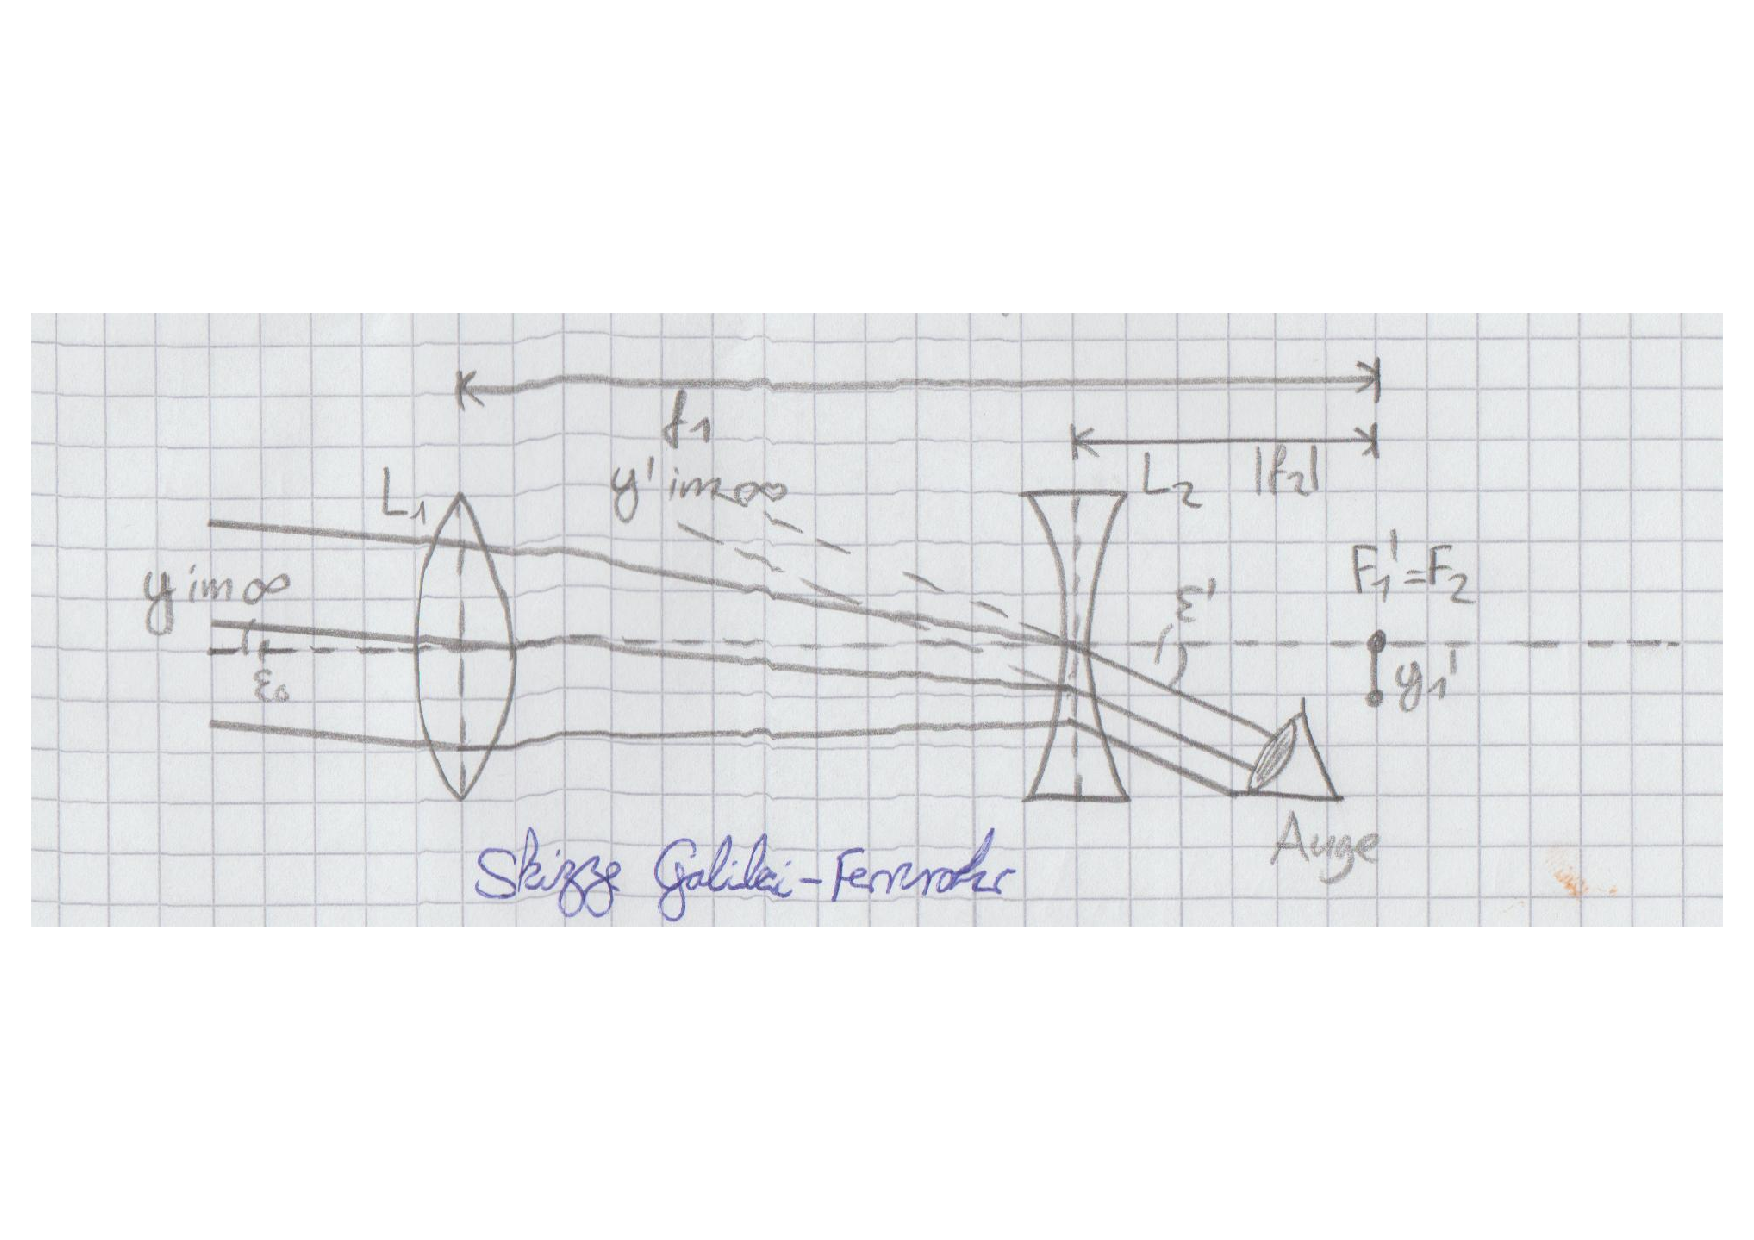
\includegraphics[width=0.9\textwidth]{./Bilder/og6}
\end{figure}
\FloatBarrier
			\\
			\(L_{1}\) funktioniert wie beim astronomischen Fernrohr, jedoch wird vor der Brennebene bereits eine Zerstreuungslinse \(L_{2}\) mit negativer Brennweite \(f_{2}\) so platziert, dass \(F'_{1}\) und \(F_{2}\) zusammenfallen. Somit beobachtet man auch hier, wie schon beim astronomischen Fernrohr ein virtuelles Bild im Unendlichen, nun jedoch richtig herum. Somit ergibt sich für das Galilei-Fernrohr die selbe Vergrößerung wie schon für das astronomische Fernrohr, wenn ihre Beträge von \(f_{1}\) und \(f_{2}\) gleich sind:
			\begin{align*}
			V_{gal}=\frac{f_{1}}{|f_{2}|}
			\end{align*}
			\\
			Mikroskop:\\
			\\
			Mit einem Mikroskop werden kleine Objekte vergrößert betrachtet, dabei vergrößert es wieder den Sehwinkel unter dem ein Gegenstand dem Betrachter erscheint. Ein Mikroskop besteht aus zwei Linsensystemen, die das Objekt abbilden. Zuerst erzeugt ein Objektiv ein vergrößertes Zwischenbild, welches durch das Okular vergrößert betrachtet wird. Das hat zur Folge, dass der Betrachter ein vergrößertes virtuelles Bild wie bei einer Lupe erkennt. Dabei befindet sich das Objekt geringfügig außerhalb der Brennweite des Objektivs \(F_{1}\), wodurch ein reelles Zwischenbild erzeugt wird, welches erheblich größer, als der eigentliche beobachtete Gegenstand ist. Das Okular wird dann so angeordnet, dass das Zwischenbild innerhalb von \(f_{2}\) nahe von \(F_{2}\) liegt (siehe Skizze).\\
			\\
	\begin{figure}[h]
\centering
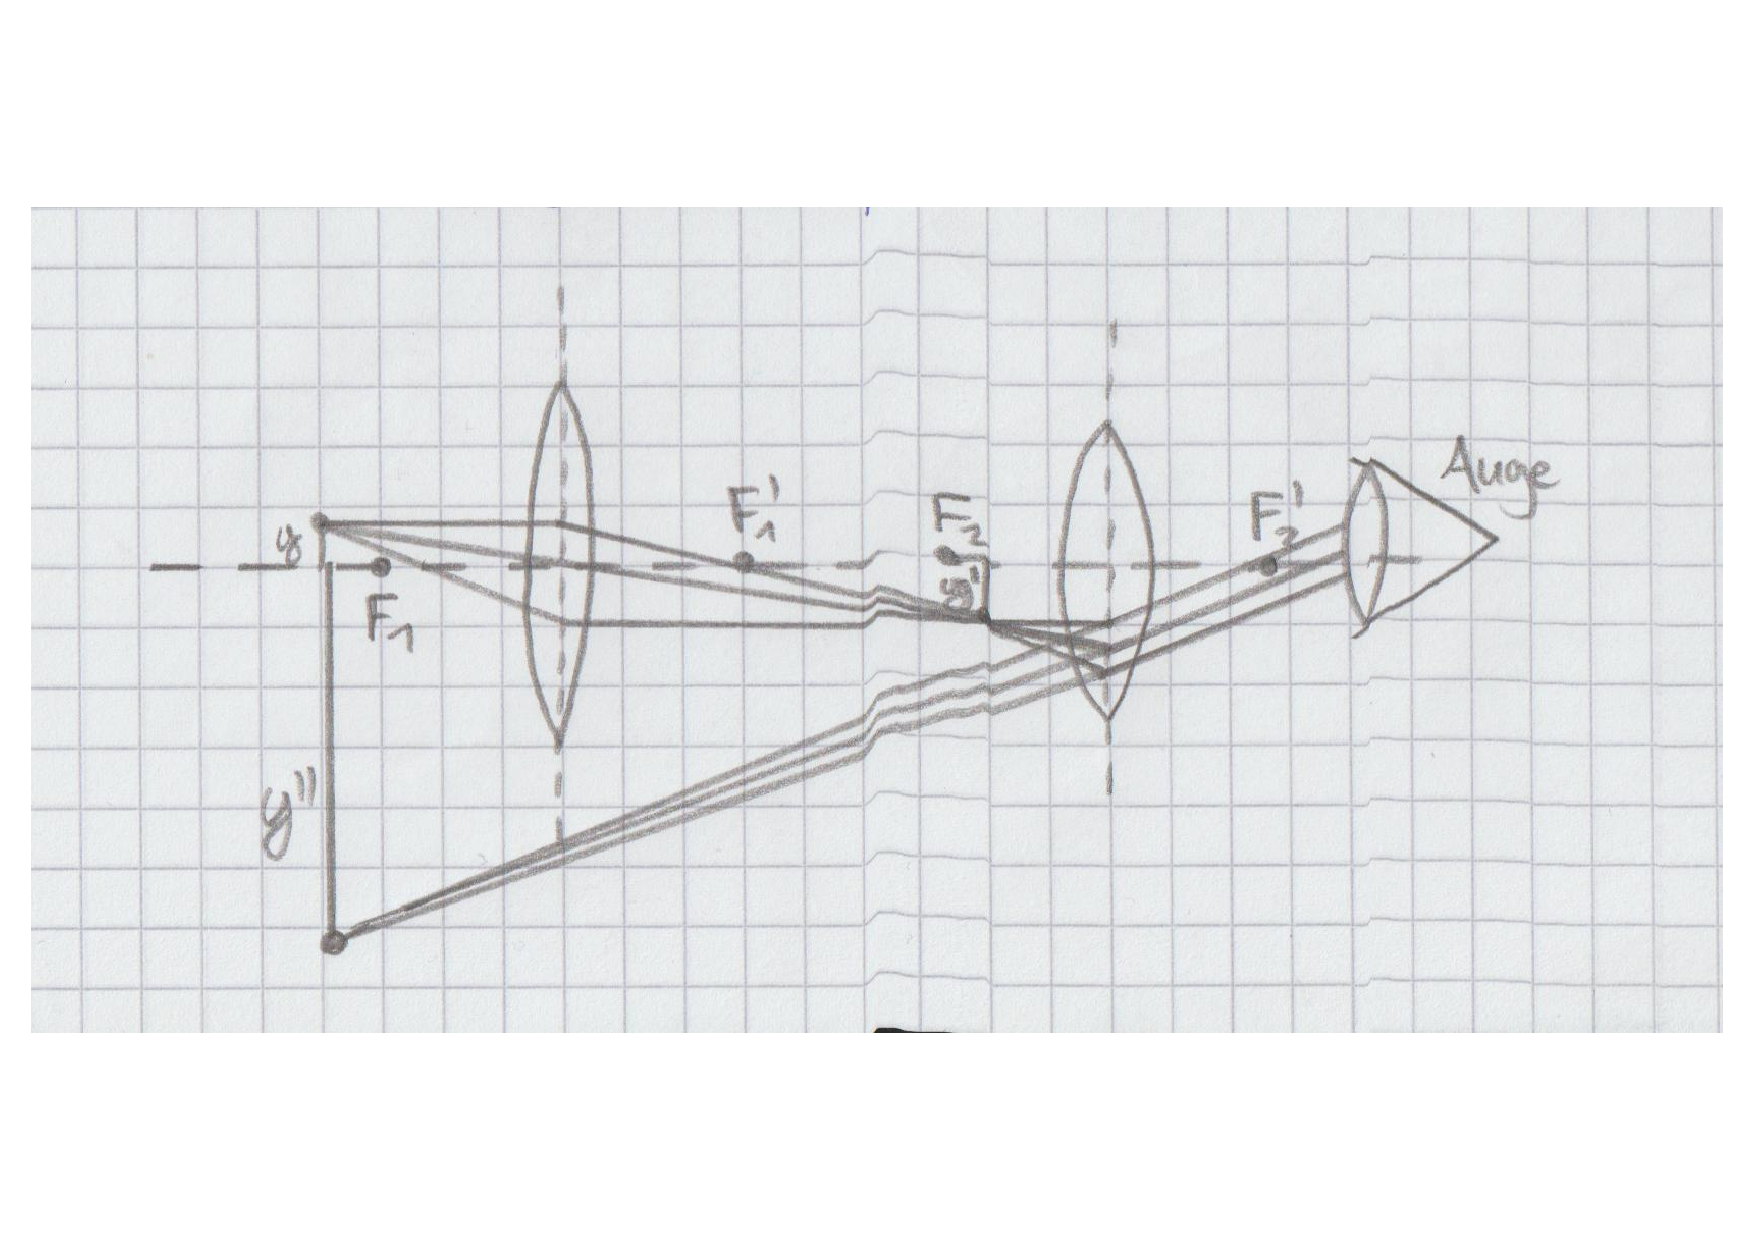
\includegraphics[width=0.9\textwidth]{./Bilder/og7}
\end{figure}
\FloatBarrier			\\
			Somit wirkt das Okular als Lupe, wodurch das Zwischenbild als virtuelles Bild \(y''\) gesehen wird. Je nach Einstellung erscheint das Objekt dann im Unendlichen oder in \(S=250mm\). Somit ergibt sich für die Gesamtvergrößerung des Mikroskops durch das Produkt der Einzelvergrößerungen
			\begin{align*}
			V_{M}=\frac{y''}{S}\frac{S}{y}=\frac{y''}{y}
			\end{align*}
			
			\newpage
			
		\subsection{Frage 4}
			In welche Entfernungsbereiche - bezogen auf die Brennweite der Lupe - können der zu betrachtende
			Gegenstand und das Auge gebracht werden?\\
			\\
			Dies ist in Aufgabe 3 unter dem Abschnitt der Lupe ersichtlich.
			
		\subsection{Frage 5}
			Warum benutzt man in der Praxis meist Prismenfernrohre? Zeichnen Sie den Strahlengang!\\
			\\
			Man benutzt heutzutage in der Praxis zumeist Prismenfernrohre, da Fernrohre, wie das Galilei-Fernrohr nur eine relativ geringe Vergrößerung ermöglichen und außerdem relativ groß sein müssen. Zudem weisen sie Linsenfehler auf. Prismenfernrohre hingegen sind sehr platzsparend und daher praktischer konstruiert.\\
			\\
	\begin{figure}[h]
\centering
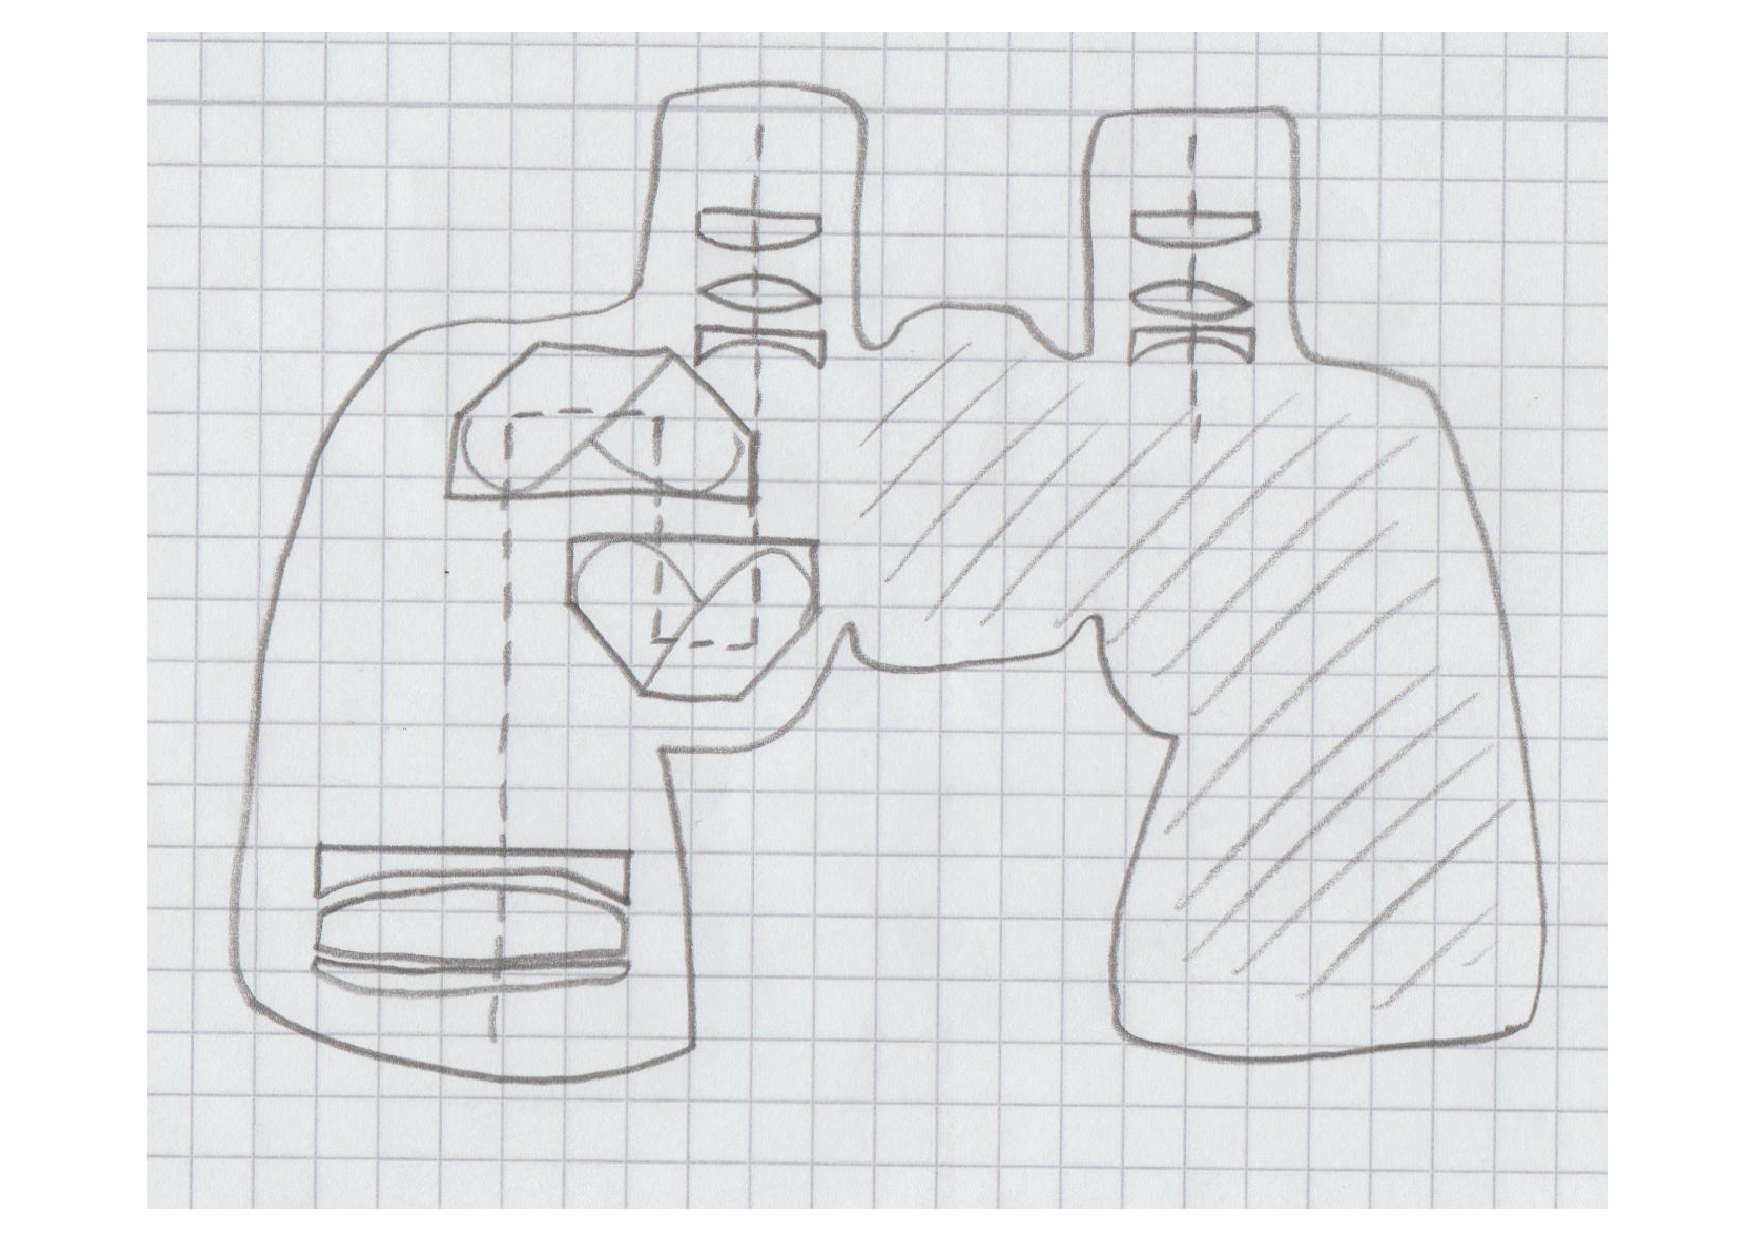
\includegraphics[width=0.9\textwidth]{./Bilder/og1}
\end{figure}
	\begin{figure}[h]
\centering
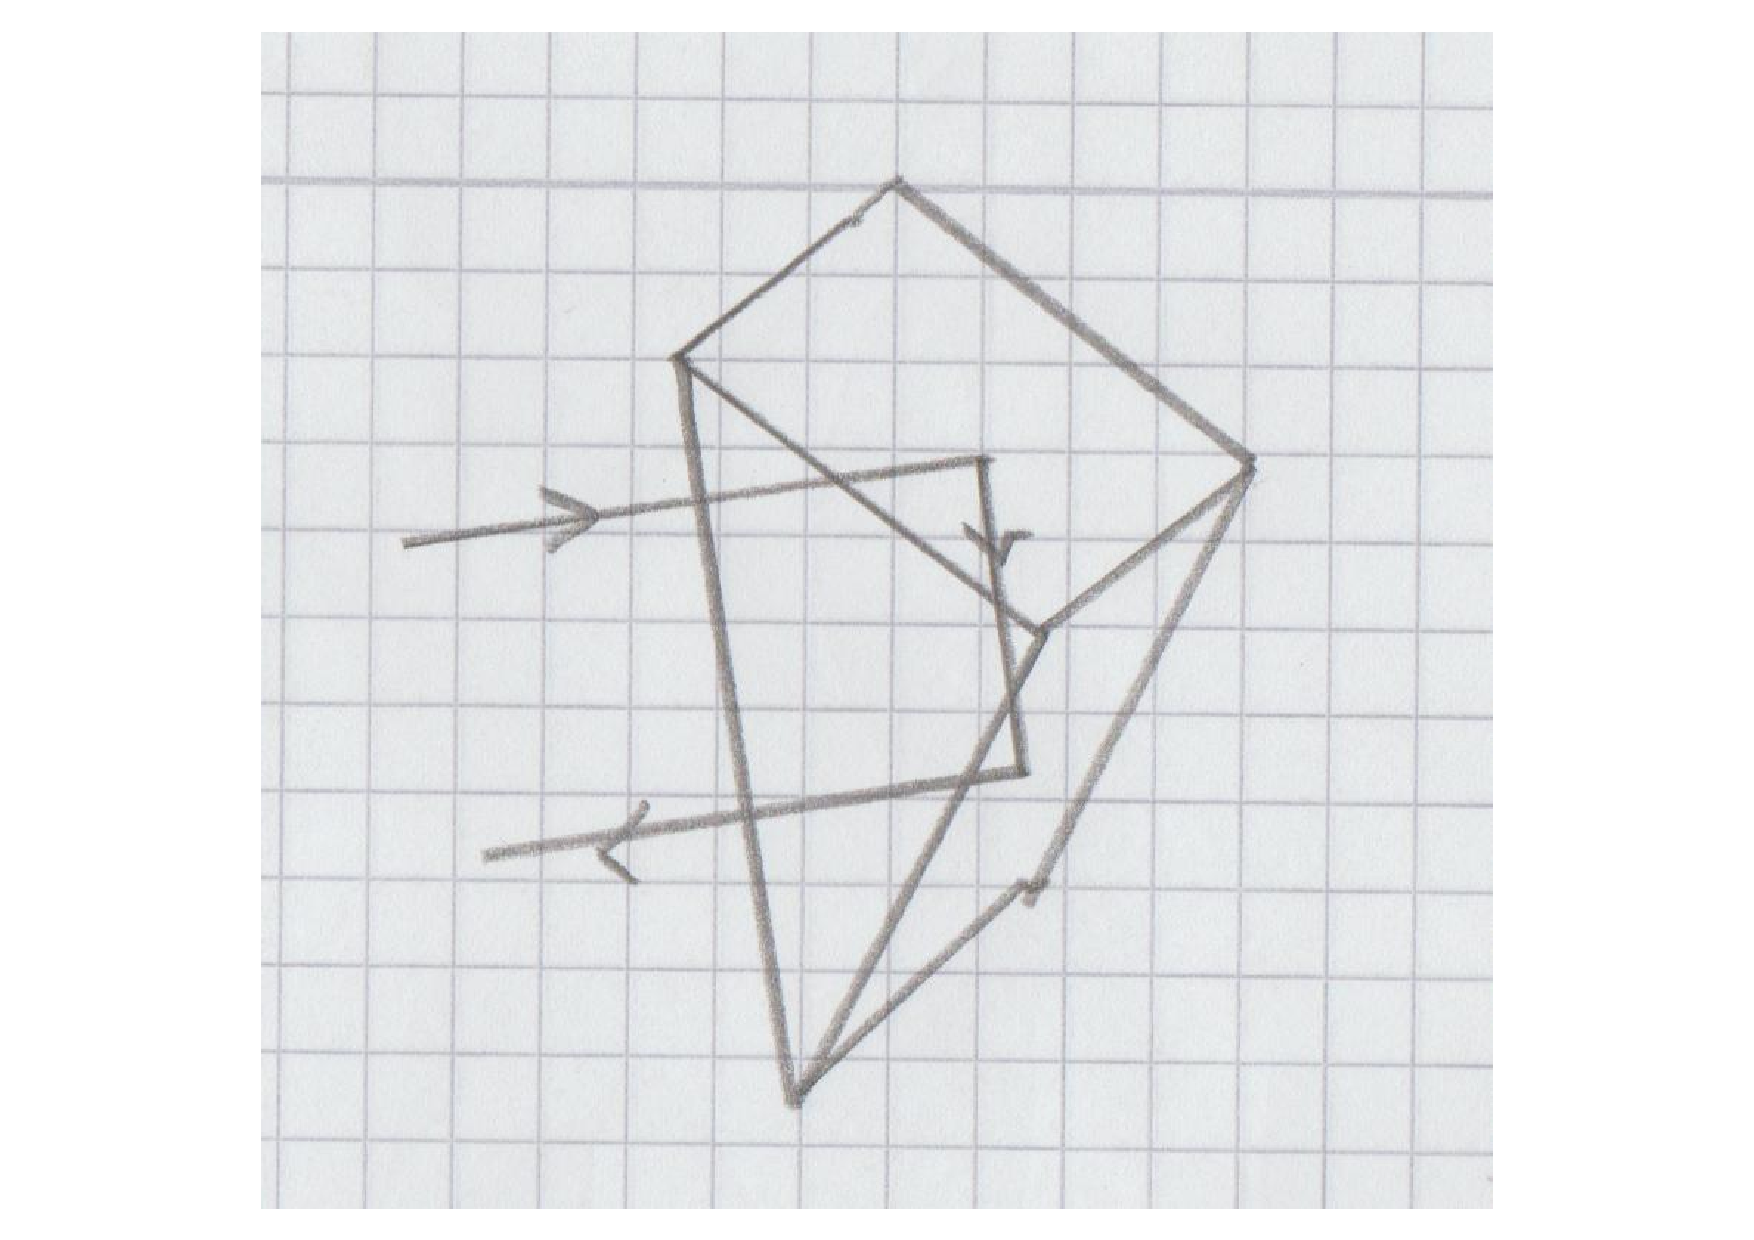
\includegraphics[width=0.9\textwidth]{./Bilder/og2}
\end{figure}
\FloatBarrier
\FloatBarrier			\\
			
		\subsection{Frage 6}
			Erläutern Sie anhand einiger einfacher optischer Abbildungsanordnungen die Begriffe Apertur und
			Gesichtsfeldblende. Was will man mit ihnen bezwecken?\\
			\\
			Es ist sehr wichtig, die Strahlenbündelbegrenzung durch Blenden zu beachten, weil durch sie Bildhelligkeit, Abbildungsfehler, Auflösungsvermögen und Schärfentiefe der Abbildung beeinflusst und verändert werden können. Eine sogenannte Aperturblende beeinflusst die Helligkeit eines Bildes gleichmäßig durch Begrenzung der Apertur (Öffnungsweite) der optischen Geräte. Sie hat jedoch keinerlei Auswirkungen auf die Größe des Bildes. Ein Beispiel dafür ist die Linsenfassung (siehe Skizze). Wenn eine Aperturblende vor der Linse angebracht ist, dringen alle Strahlen durch die Blende in das System ein. Somit wird die Aperturblende wie ein Gegenstand abgebildet, wobei alle aus dem System austretenden Strahlen durch das virtuelle Bild der Aperturblende begrenzt werden. Häufig ist die Aperturblende zwischen zwei Linsen angebracht. Ein Beispiel für Aperturblenden aus der Natur stellt die Iris des menschlichen Auges dar.\\
			\\
				\begin{figure}[h]
\centering
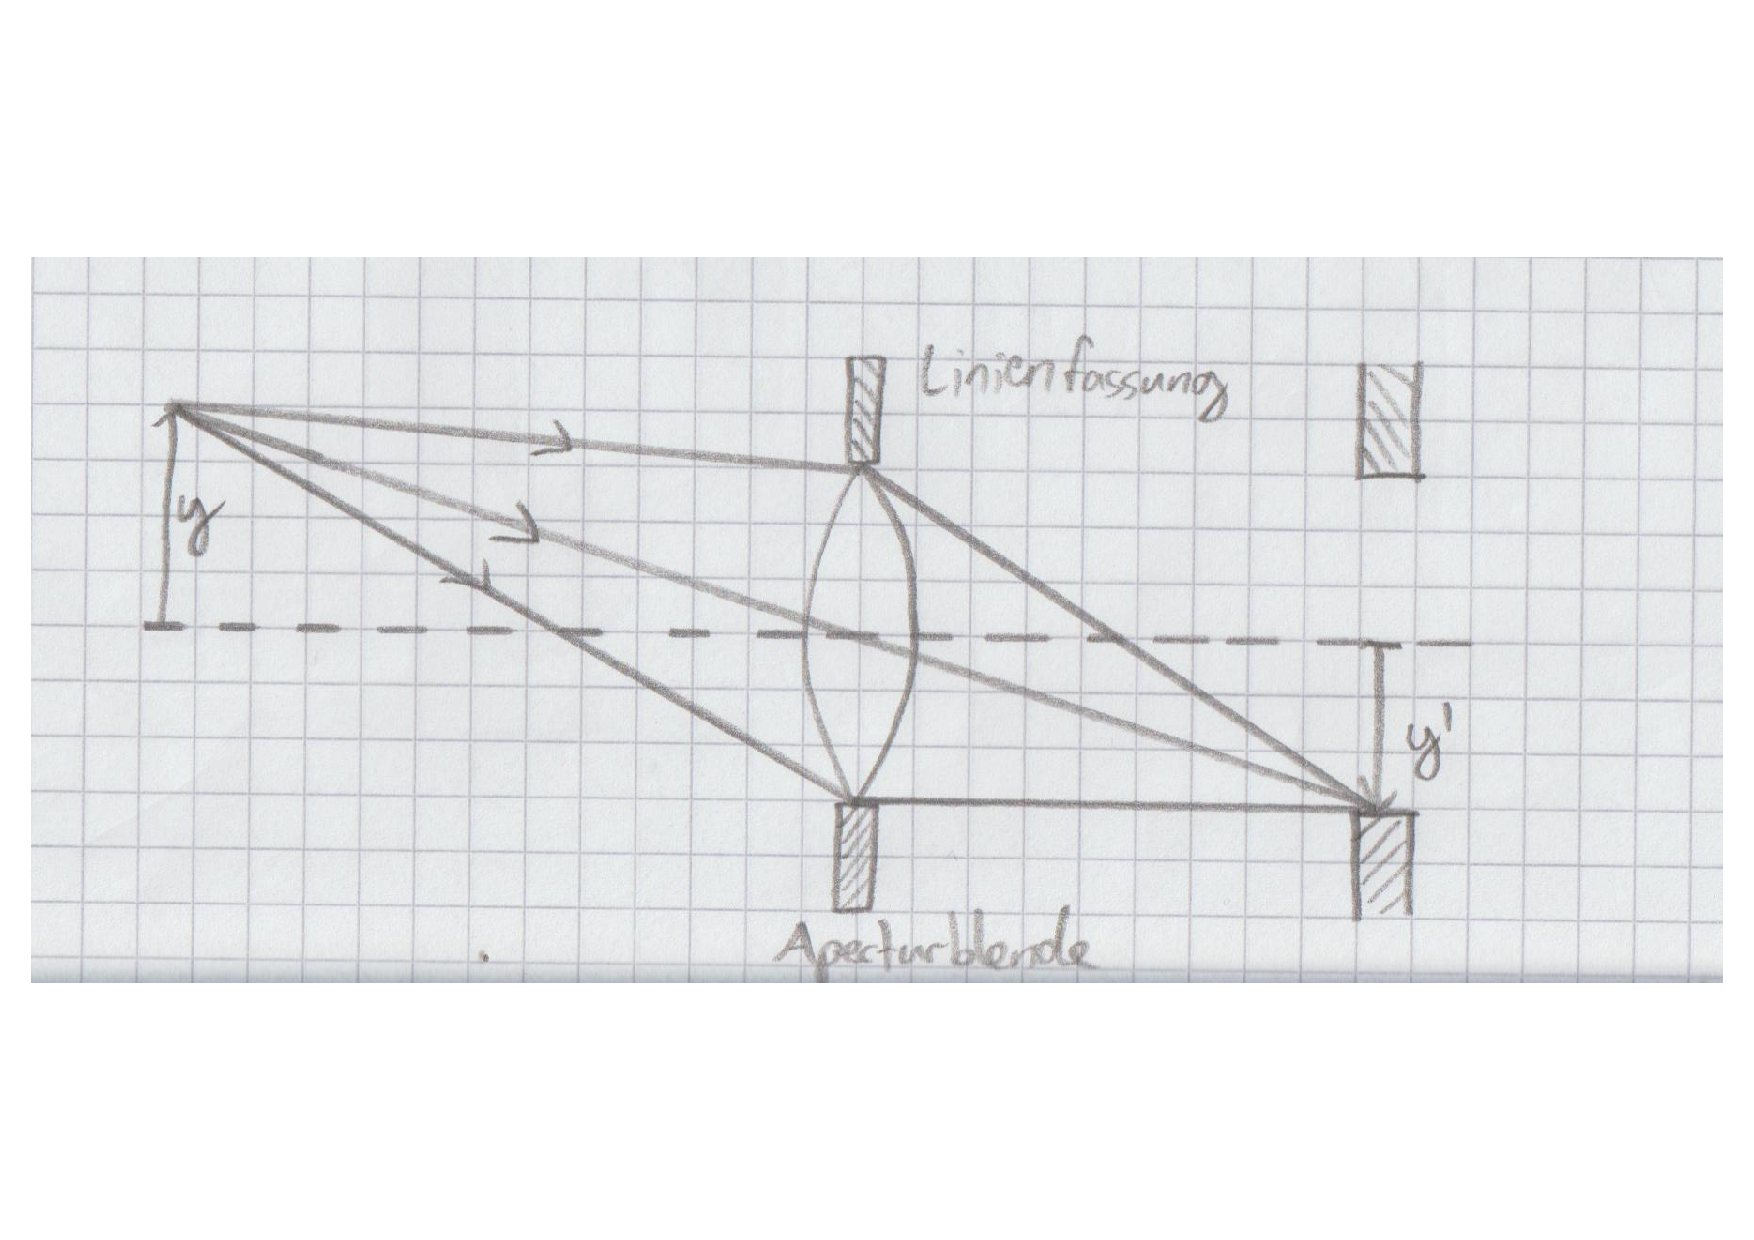
\includegraphics[width=0.9\textwidth]{./Bilder/og3}
\end{figure}
\FloatBarrier
			\\
			Eine Gesichtsfeldblende hingegen hat keine Auswirkung auf die Helligkeit eines Bildes, begrenzt jedoch den Bildausschnitt. Sie wird in der Bildebene plaziert oder in der Objektebene. Falls das Bild ein Diapositiv ist, ist die Dia-Maske die Feldblende, die den projizierten Bildausschnitt festlegt. Die Feldblende kann bei mehrstufiger Abbildung aber auch in der Ebene eines Zwischenbilds liegen. Das ist beim Mikroskop z.B. der Fall. \\
			\\
	\begin{figure}[h]
\centering
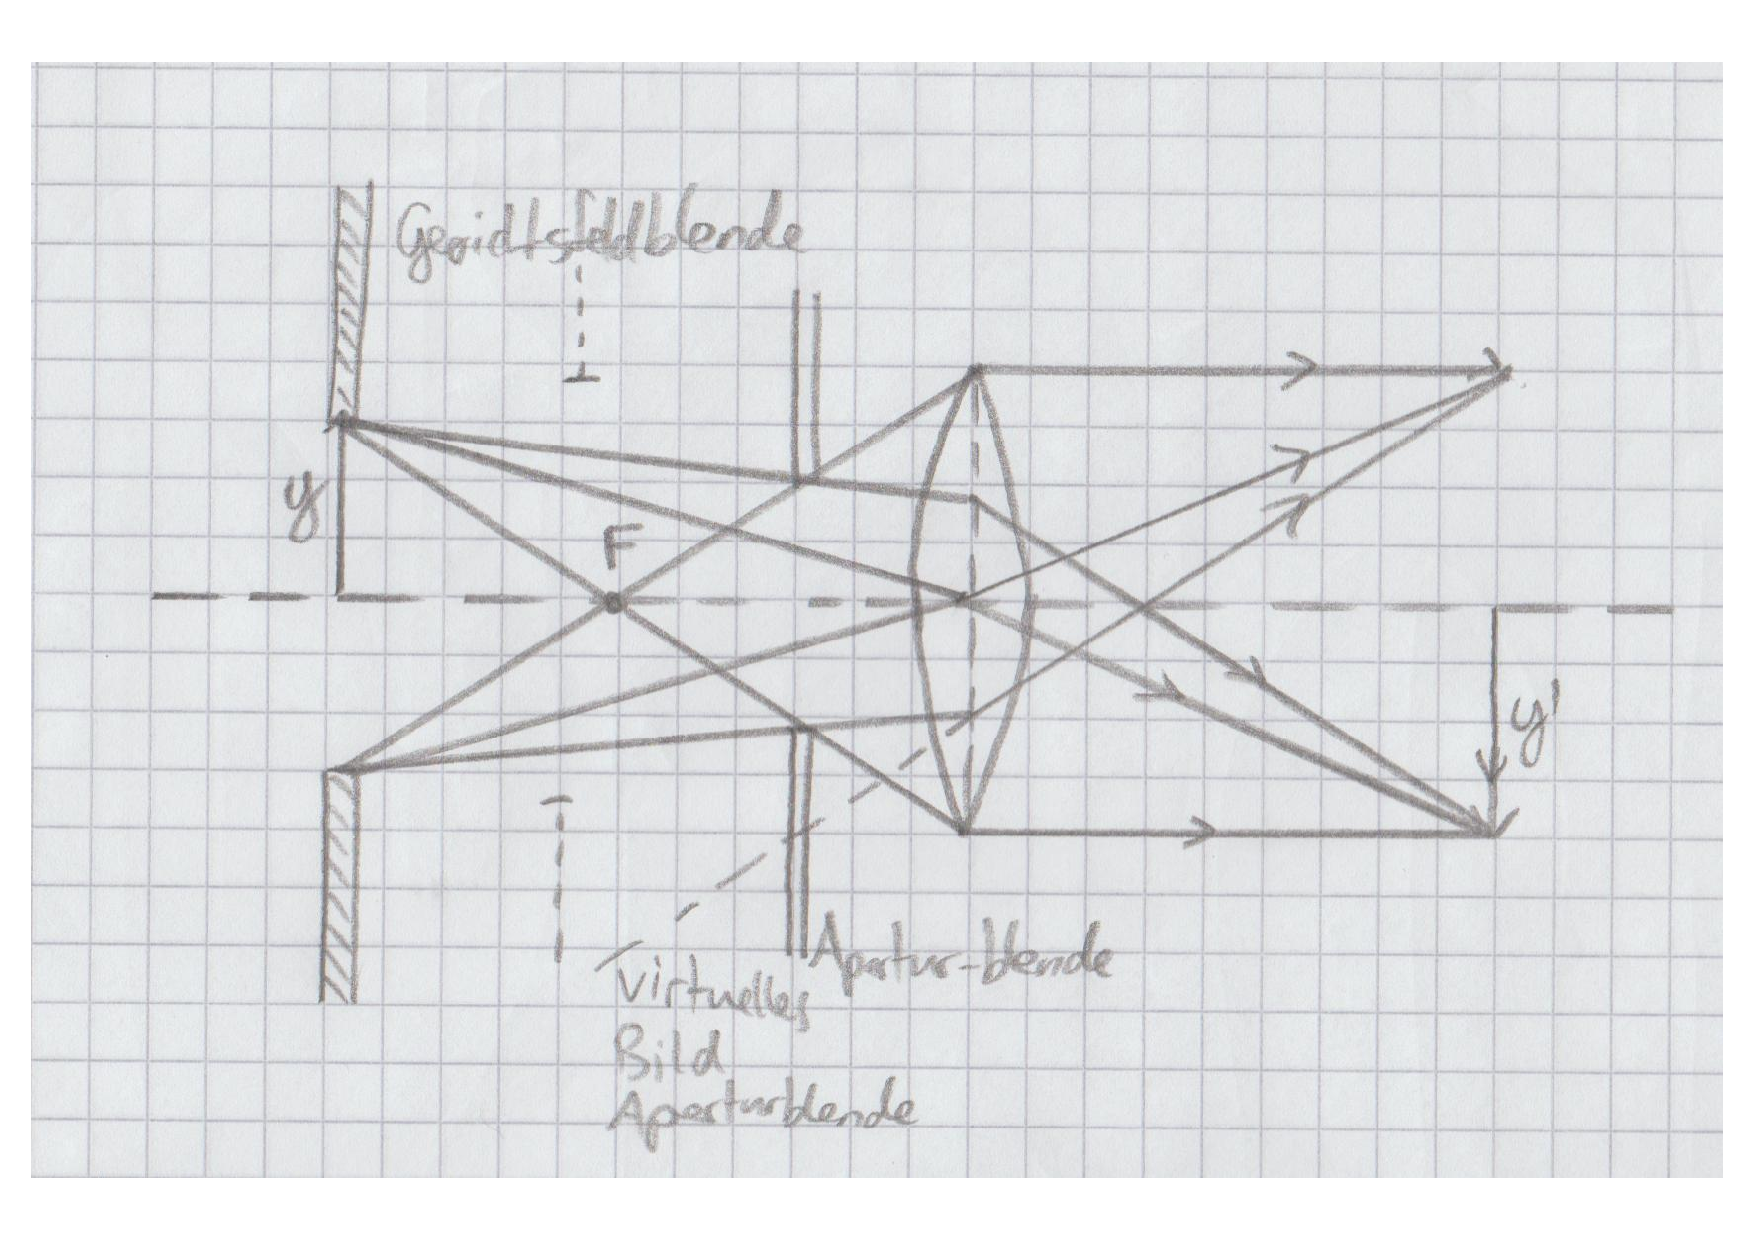
\includegraphics[width=0.9\textwidth]{./Bilder/og14}
\end{figure}
\FloatBarrier			\\
			
		\subsection{Frage 7}
			Wie lassen sich in optischen Systemen mit einem vorgegebenen Linsensatz kurze Brennweiten
			erzielen?\\
			\\
			Durch kleinere Blendendurchmesser und größere Blendenzahl lassen sich in optischen Systemen mit vorgegebenem Linsensatz kurze Brennweiten erzielen.
			
			\subsection{Frage 8}
		Welche Linsenfehler gibt es? Nennen Sie Möglichkeiten zu ihrer Beseitigung!
		\\
		\\
		Eine sphärische Linse bildet einen Gegenstandspunkt nur dann in guter Näherung in einen Bildpunkt ab, wenn man die Bedingungen des Paraxialgebietes (nur achsennahe Strahlen werden betrachtet) einhält. Um unabhängig von Dispersion, darf nur monochromatisches Licht verwendet werden (Laser erfüllt diese Bedingung in guter Näherung). Bei Abbildungen mit weißem Licht kommt es zu Farbfehlern (chromatische Aberration), auch im Paraxialgebiet. Es entstehen Bilder mit unscharfen, farbigen Rändern. Aus einem achsenparallelen, monochromatischen Strahlenbündel werden umgekehrt durch eine Sammellinse nur die achsennahen Strahlen in einem Brennpunkt gesammelt, die Randstrahlen jedoch in einem näher an der Linie liegenden Punkt. Dem verschiedenen Brennweiten und einhergehenden Bildweiten entsprechend, entsteht ein unscharfes Bild. Man spricht vom Öffnungsfehler oder sphärische Aberration, der durch den Einsatz von Blenden verringert werden kann.
	
			
	
		\begin{itemize}
			\item Bildfeldwölbung: Ein ebener Gegenstand wird von einer dünnen (plankonvexen) Einzellinse in eine gekrümmte Bildfläche abgebildet. Dieser Fehler lässt sich durch eine bikonvexe Linse oder einen entsprechend gewölbten Schirm vermeiden
		
				
		
			\item Verzeichnung: Eine tonnenförmig Verzeichnung eines Gitters entsteht, wenn eine strahlenbegrenzende Blende zwischen Gegenstand und Linie liegt. Eine kissenförmige Verzeichnung findet man, wenn eine Blende zwischen Linse und Bild steht. Beide Fehler heben sich gewissermaßen gegenseitig auf.
		
				
			
			\item Koma: Bei Abbildung eines Punktes, der außerhalb der Achse einer Linse liegt, welche sphärische Aberration besitzt überschneiden sich die Strahlen zum Teil schon vor der Bildebene, Anstelle eines scharfen Punktes entsteht ein Bild mit einem einseitig radial gerichteten kometenhaften Schwanz: Koma. Die Störung ist umso größer umso größer, je schiefer der Einfall und je größer die Linsenöffnung ist und kann entsprechend durch achsenparallele Ausrichtung der Strahlen und Begrenzung der Öffnung durch eine Blende verringert werden
			
				
	
			Durch Kombination mehrerer ausgewählter Konvex- und Konkavlinsen aus verschiedenen Glasarten zu einem Linsensystem lassen sich Abbildungsfehler erheblich reduzieren. Andererseits treten Abbildungsfehler nicht unabhängig voneinander voneinander auf, eine gleichzeitige Korrektur aller Fehler ist nicht möglich. Ferner lassen sich Linsenfehler z. T. durch Verwendung asphärisch geschliffener Linsen deutlich reduzieren.
		\end{itemize}	
	\subsection{Frage 9}
		Erläutern Sie, warum Präzisionsfernrohre für die Astronomie nicht mit Linsen sondern mit Spiegeln gebaut werden.
		\\
		\\
		Präzisionsfernrohre für die Astronomie werden mit Spiegeln, nicht mit Linsen gebaut, um Farbfehler zu vermeiden, da das Licht mithilfe der Spiegel reflektiert, nicht gebrochen wird. Außerdem ist beinahe eine beliebige Baugröße möglich, da das Licht nicht wie bei Linsen durch die Spiegel hindurch strahlt. Die Spiegel können somit rückwärtig gestützt werden.
	\subsection{Frage 10}
		Zeichnen und erläutern Sie die Optik im menschlichen Auge! Erörtern Sie Kurz- undWeitsichtigkeit sowie Astigmatismus.
		\\
		\\
		Das optische Instrument Auge, das nahezu eine Kugel mit Radius $r\approx12 mm$ ist, besteht im Wesentlichen aus der lichtempfindlichen Netzhaut sowie aus einem Linsensystem, das aus der Hornhaut, der vorderen Augenkammer und der Linse gebildet wird, Die Brechkraft $D=\frac{1}{f}$ dieser Linse wird durch Muskeln geregelt. Die Linse mit einem Durchmesser von $10 mm$ beim Erwachsenen ist durch Zonulafasern in der hinteren Augen aufgehängt. Die Regenbogenhaut bildet eine lichtdurchlässige Öffnung, die Pupille, die wie eine Blende den gesamten Lichtfluss in das Auge regelt. Der Durchmesser der Pupille $d$ kann zwischen ca. $2 mm$ (Tagsehen) und $7,5 mm$ (Nachtsehen) variieren. Die Sehschärfe des Auges ist bei $d=3 mm$ am größten, da bei größeren Werten bereits Farbfehler und sphärische Aberration eine Rolle spielen. Die optimale Abbildung im Auge erfolgt auf die Netzhaut, die mit speziellen Lichtempfängern, den Stäbchen für das Nachtsehen und den Zapfen für das Farbsehen, ausgestattet ist.
		
			\begin{center}
				\begin{figure}[h]
\centering
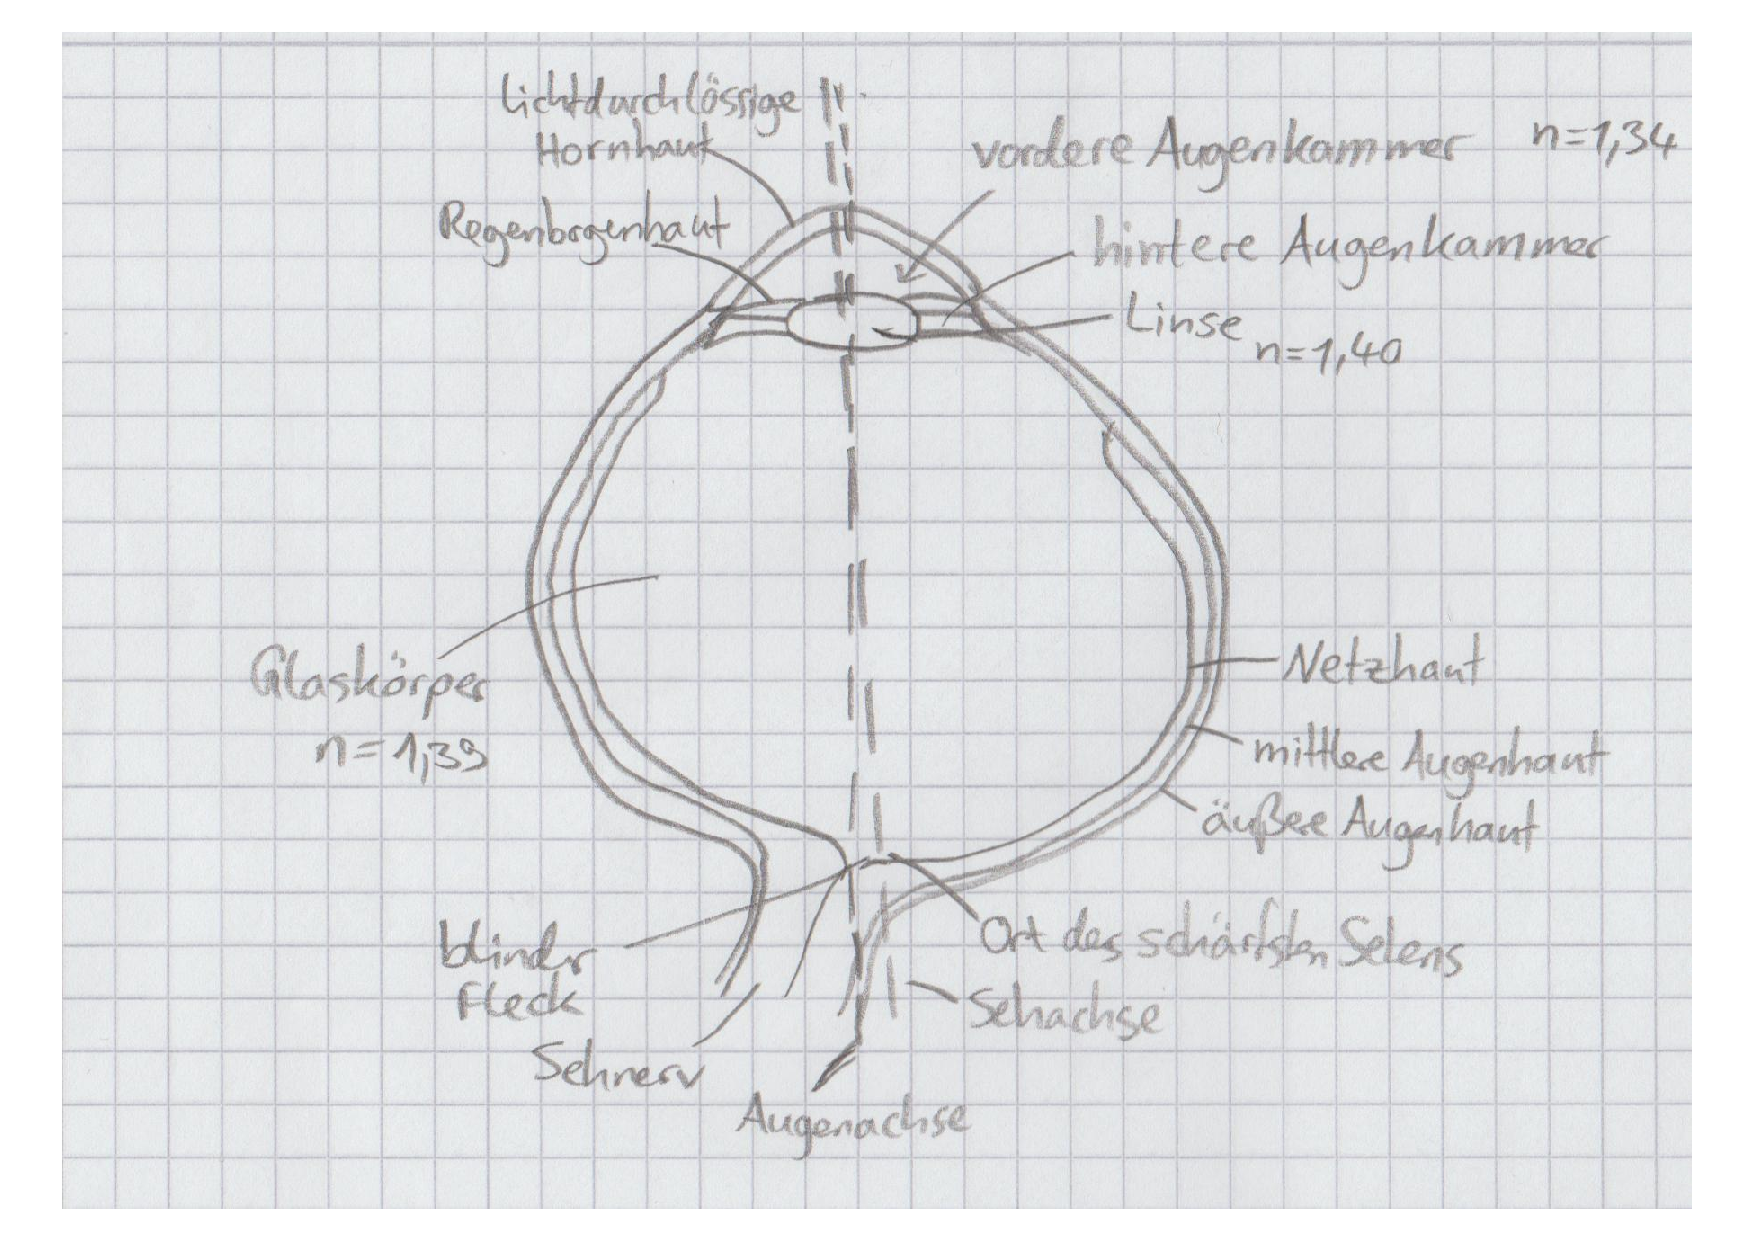
\includegraphics[width=0.9\textwidth]{./Bilder/og13}
\end{figure}
\FloatBarrier
			\end{center}
	
		\begin{itemize}
			\item Kurzsichtigkeit: Wenn der Glaskörper des Auges zu lang ist beziehungsweise die Augenlinse zu krumm, so wird das Bild weit entfernter Objekte nicht auf der Netzhaut sondern kurz davor scharf abgebildet. Auf der Netzhaut ergibt sich ein unscharfes Bild. Kurzsichtige Menschen können weit entfernte Gegenstände nur unscharf sehen. Hier hilft eine Brille mit Zerstreuungslinse.
			\item Weitsichtigkeit: Wenn der Glaskörper des Auges zu kurz ist beziehungsweise die Augenlinse nicht krumm genug, so wird das Bild naher Gegenstände nicht auf der Netzhaut, sondern erst kurz dahinter scharf abgebildet. Auf der Netzhaut ergibt sich daher ein unscharfes Bild. Weitsichtige Menschen können nahe Objekten nur unscharf sehen, Hier hilft eine Brille mit Sammellinse.
			\item Astigmatismus: Beim Astigmatismus (Punktlosigkeit) kommt es aufgrund einer Hornhautverkrümmung zu einer unterschiedlichen Ablenkung einfallender Strahlen. Diese treffen sich bei einem (schräg einfallenden) Parallelbündel nicht in einem Punkt, sondern auf zwei Brennlinien, dem vertikalen Meridionalschnitt und dem horizontalen Sagittalschnitt.
			
					\begin{figure}[h]
\centering
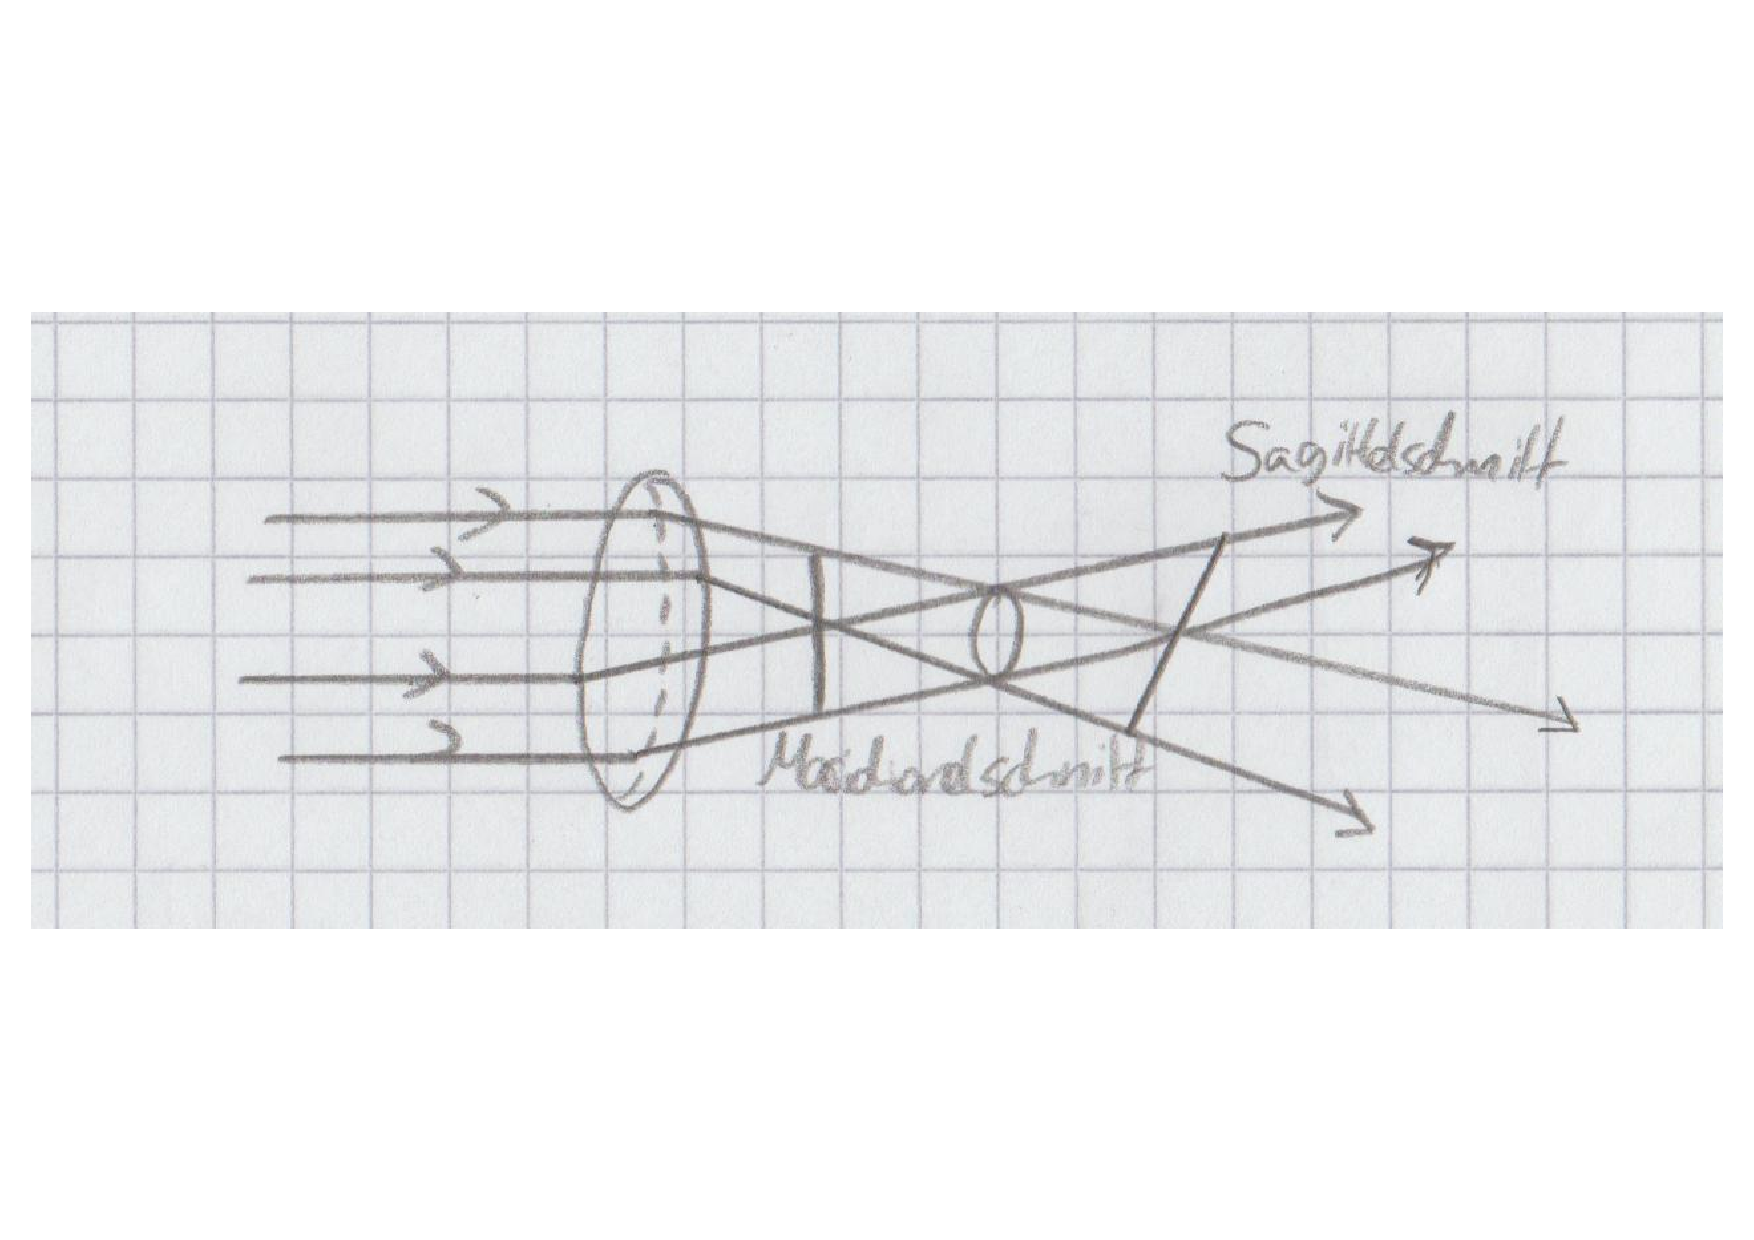
\includegraphics[width=0.9\textwidth]{./Bilder/ogmarcostinkt}
\end{figure}
\FloatBarrier
	
				Astigmatismus bei Fokussierung eines Parallelbündels durch eine schräg gestellte Linse
		\end{itemize}
	\subsection{Frage 11}
		Warum besteht der Kondensor eines Diaprojektors aus zwei plankonvexen Linsen? (Hinweis: Berücksichtigen Sie die Reflexionsverluste!)
		\\
		\\
		Ziel und Zweck des Kondensors beim Diaprojektor ist, eine möglichst hohe Beleuchtungsstärke zu erreichen sowie möglichst geringe Reflexionsverluste. Daher besteht der Kondensor aus zwei plankonvexen Linsen, die das von der Lampe ausgestrahlte Licht in gleichmäßigen, parallelen Strahlen auf der Dia treffen lassen. Andernfalls würder es bei Betrachtung des Bildrandes zu einem Helligkeitsabfall kommen.
	\subsection{Frage 12}
		Wie kann man die Vergrößerung eines Fernrohrs ohne Kenntnis der Brennweiten messen?
		\\
		\\
		Sind die Brennweiten der Linsen eines Fernrohres nicht bekannt, kann man die Winkelvergrößerung $\Gamma_{Kep}$ beziehungsweise $\Gamma_{Gal}$ mithilfe der Gleichheit $\frac{D_{EP}}{f_{Ob}'}=\frac{D_{AP}}{f_{Ok}}$ bestimmt werden:
	
		Winkelvergrößerung der Fernrohre

			\[\Gamma_F=\frac{D_{EP}}{D_{AP}}\]
	
		wobei mit $D_{EP}$ der Durchmesser der Eintrittspupille, mit $D_{AP}$ der Durchmesser der Austrittspupille $AP$ reell hinter dem Okular abgebildet.
		
				\begin{figure}[h]
\centering
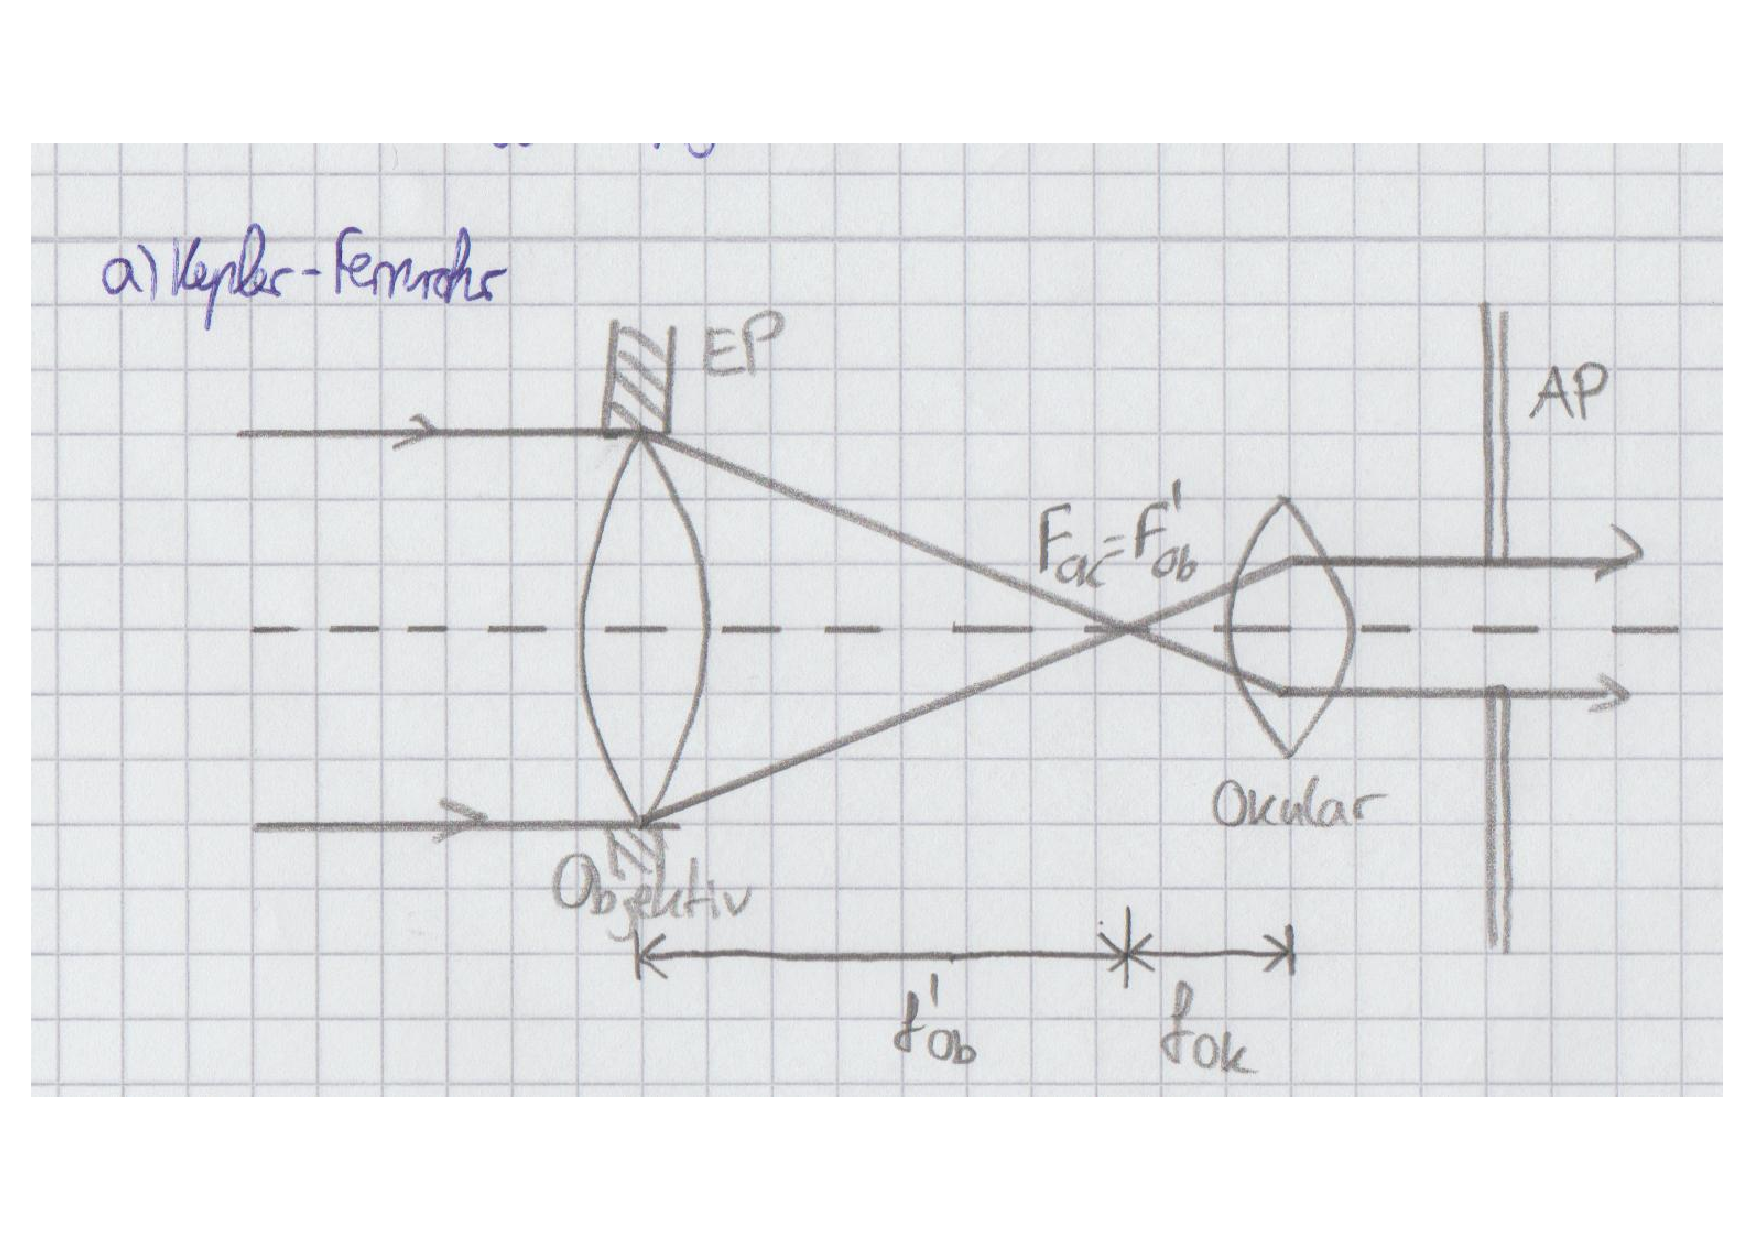
\includegraphics[width=0.9\textwidth]{./Bilder/og10}
\end{figure}
\FloatBarrier
	\begin{figure}[h]
\centering
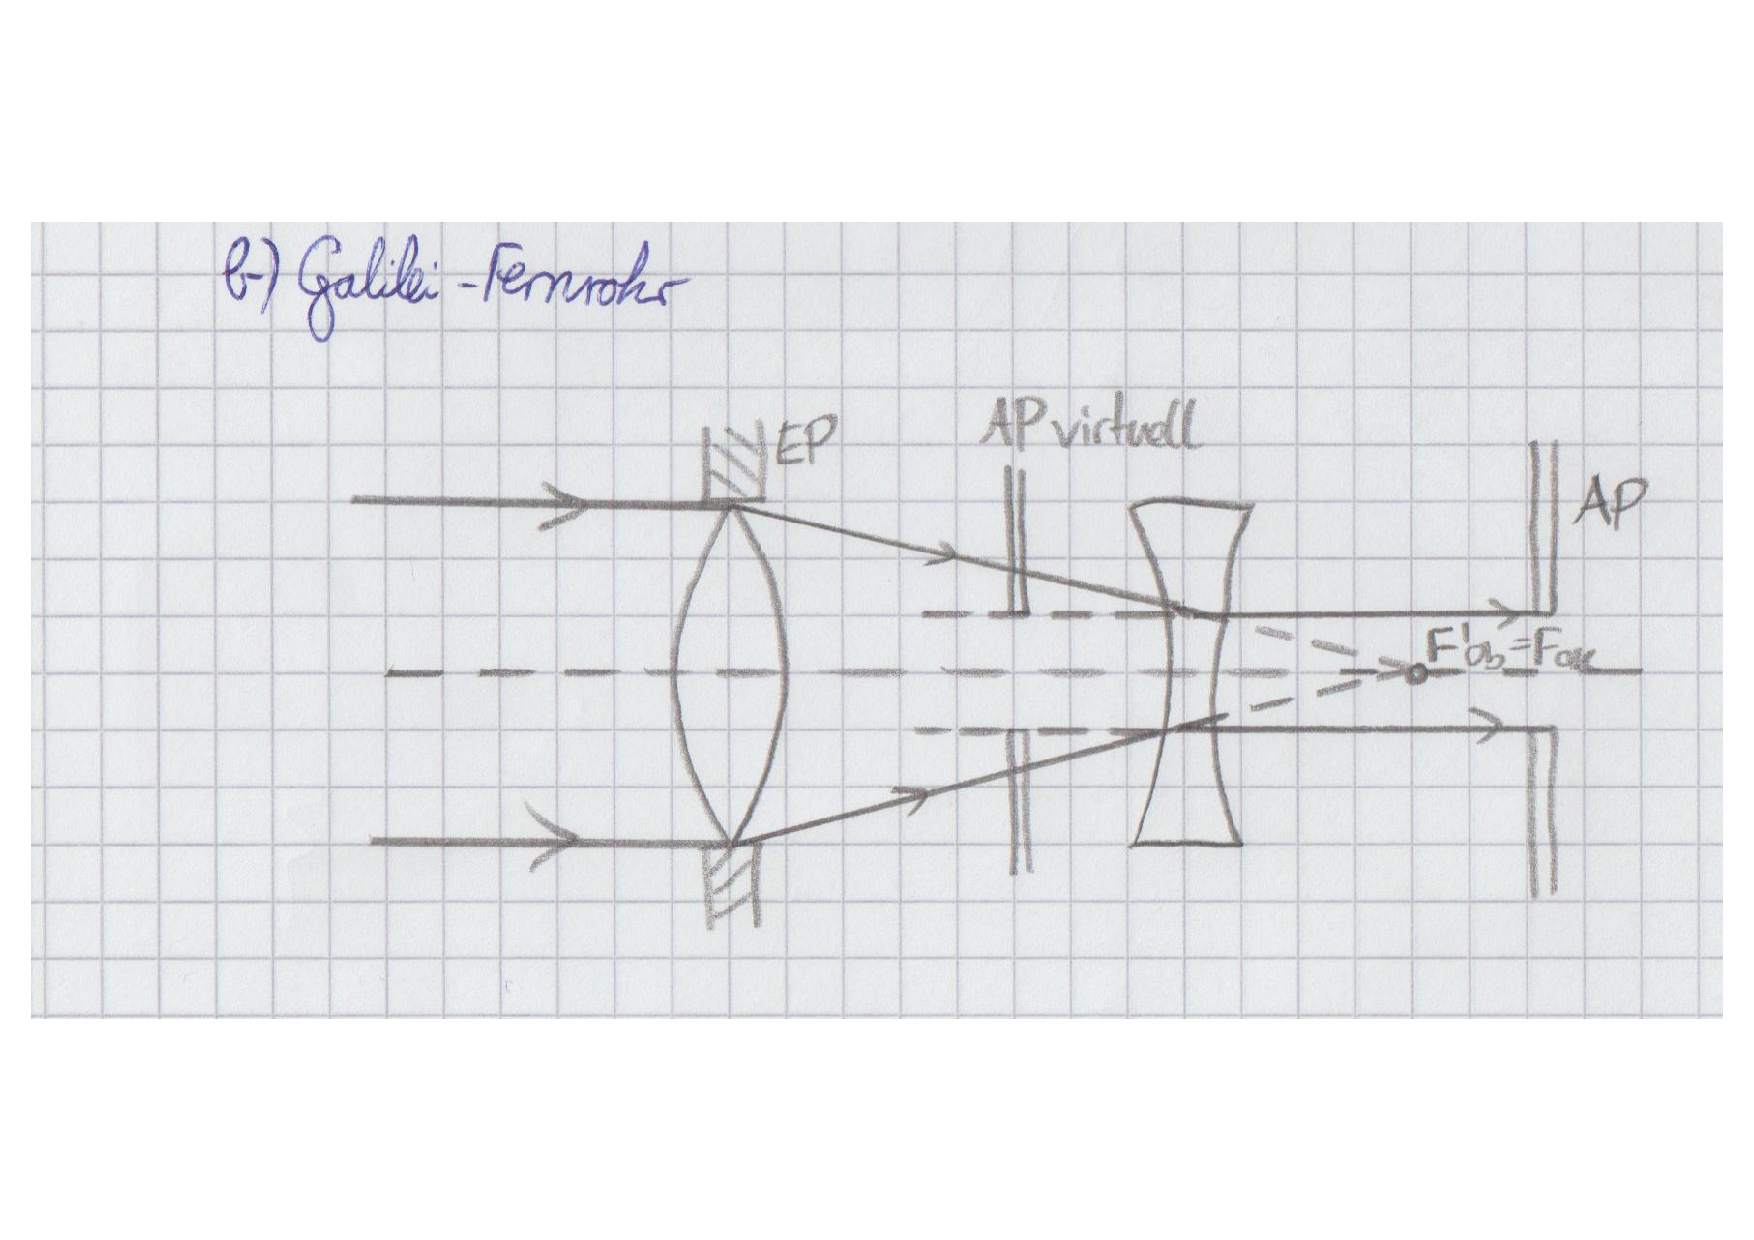
\includegraphics[width=0.9\textwidth]{./Bilder/og11}
\end{figure}
\FloatBarrier
	\subsection{Frage 13}
		Schätzen Sie die Größenordnung der Objektivbrennweite für einen Heimdiaprojektor ab, wenn Sie Raumgröße, Dia- und Leinwandgröße in Betracht ziehen.
		\\
		\\
		Die Projektionsobjektive eines Bildprojektors werden i. A. aus drei bis fünf Linsen aufgebaut. Die Linsengleichung gibt den Zusammenhang zwischen Objektivbrennweite $f$, Bildweite $a$ sowie Abbildungsmaßstab $\beta=\frac{y'}{y}=\frac{a'}{a}$ an. Wird sie für ein normales Kleinbilddis mit der projizierten Fläche $23 mm \cdot 35 mm$ ausgewertet, so ergibt sich für die Diaseite $y=35 mm$ eine Bildbreite $\left|y'\right|$ auf der Projektionswandnach folgendem Diagramm.
			\begin{figure}[h]
\centering
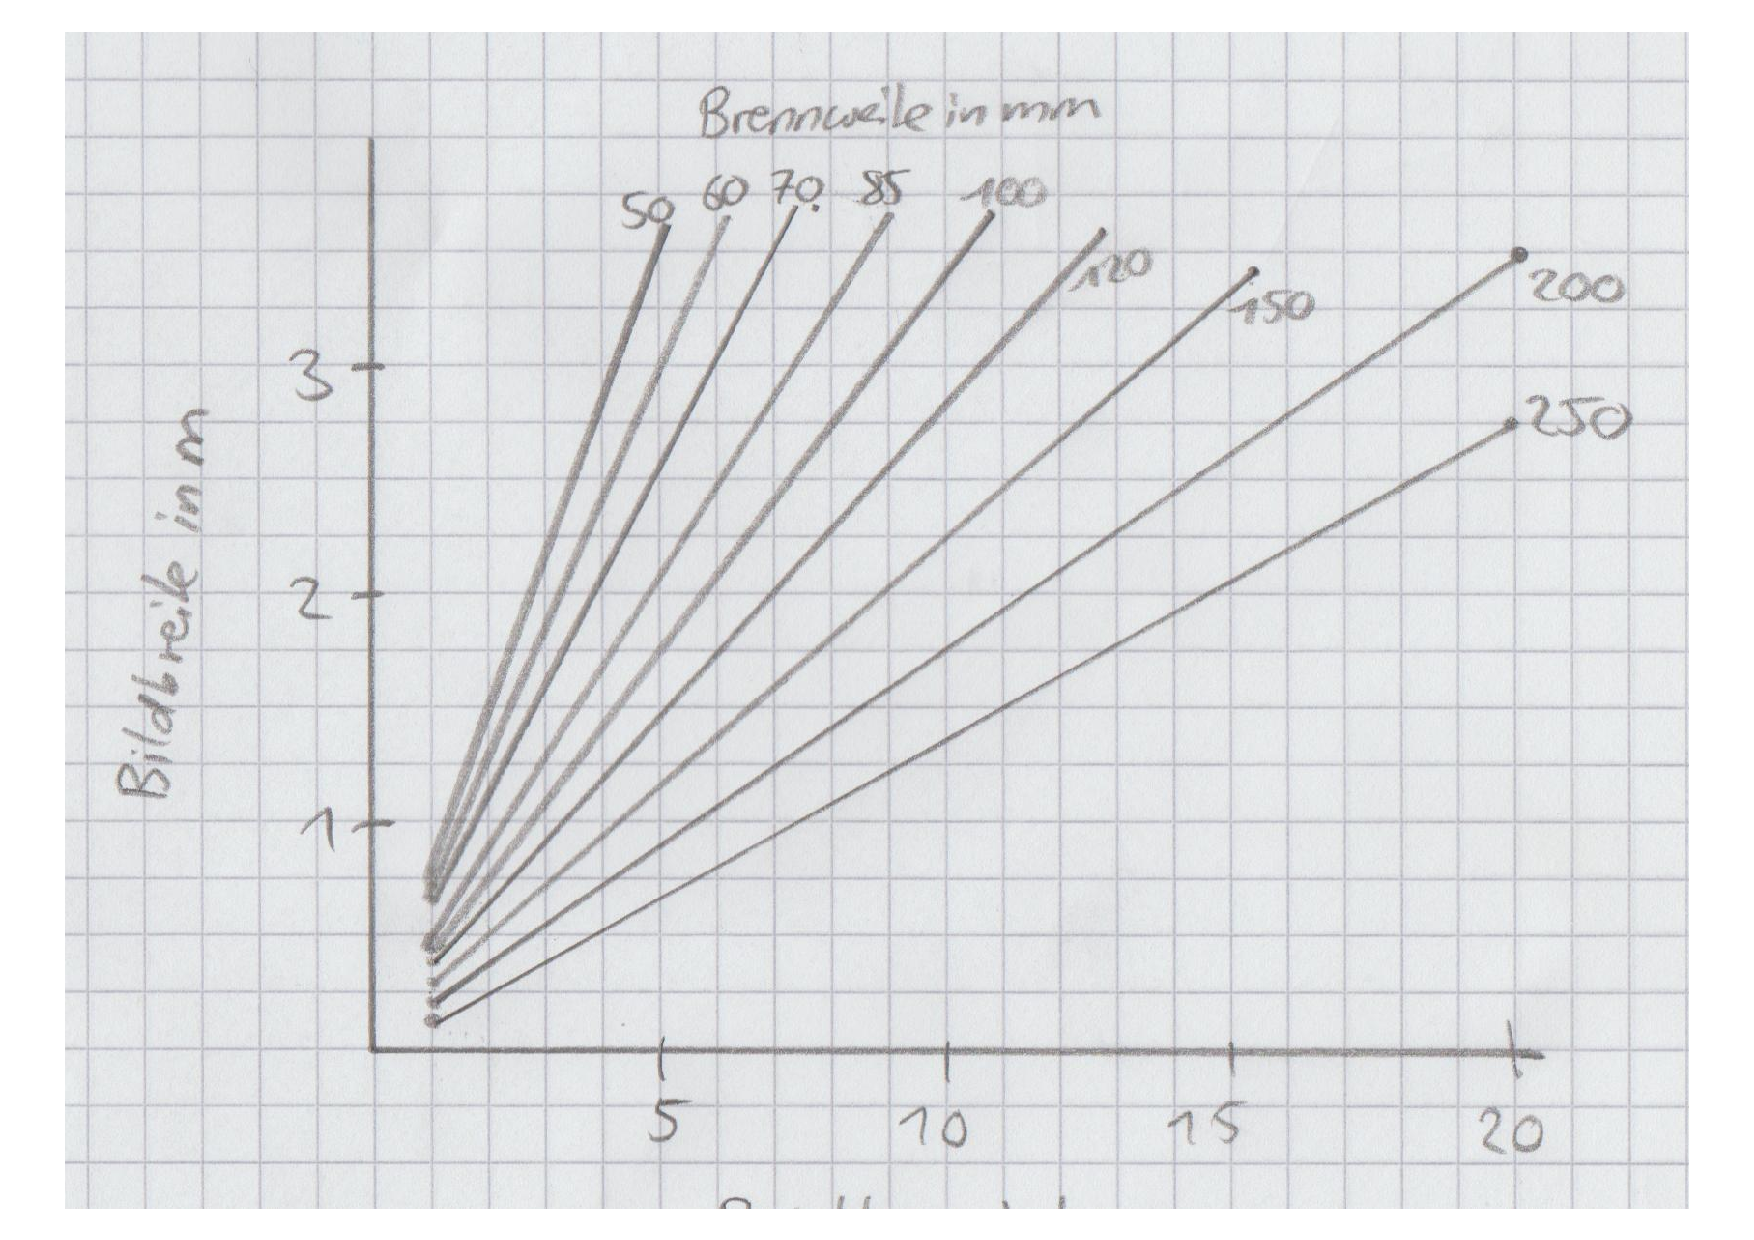
\includegraphics[width=0.9\textwidth]{./Bilder/og12}
\end{figure}
\FloatBarrier
	
			\begin{center}
			Skizze
			\end{center}
		
	\end{document}
